% partition-methods.tex: how a distributed tree is cut and moved, drawn.
% Build with make (figures.py writes the fig-*.tex files first).
\documentclass[10pt,a4paper]{article}
\usepackage[margin=2cm]{geometry}
\usepackage[T1]{fontenc}
\usepackage{lmodern}
\usepackage{amsmath}
\usepackage{amssymb}
\usepackage{amsthm}
\usepackage{booktabs}
\usepackage{array}
\usepackage{xcolor}
\usepackage{tikz}
\usetikzlibrary{arrows.meta, positioning, fit, backgrounds, patterns,
  decorations.pathreplacing, calc, shapes.misc}
\usepackage{float}
\usepackage{algorithm}
\usepackage{algpseudocode}
\algrenewcommand\algorithmicrequire{\textbf{In:}}
\algrenewcommand\algorithmicensure{\textbf{Out:}}
\algrenewcommand\algorithmiccomment[1]{\hfill{\footnotesize\color{black!60}\(\triangleright\) #1}}
\usepackage{caption}
\usepackage{subcaption}
\usepackage[hidelinks]{hyperref}
\usepackage{enumitem}
\setlist{nosep, leftmargin=1.4em}
\captionsetup{font=small, labelfont=bf}
\setlength{\parindent}{0pt}
\setlength{\parskip}{0.55em}
\theoremstyle{definition}
\newtheorem{definition}{Definition}
\newtheorem{proposition}{Proposition}

% the four ranks (Okabe-Ito, safe for colour blindness)
\definecolor{r0}{HTML}{0072B2}
\definecolor{r1}{HTML}{E69F00}
\definecolor{r2}{HTML}{009E73}
\definecolor{r3}{HTML}{CC79A7}

\newcommand{\fn}[1]{\texttt{#1}}
\input{fig-counts.tex}
\input{fig-skelcounts.tex}
\input{fig-migcounts.tex}
\input{fig-zcounts.tex}
\input{fig-wcounts.tex}
\input{fig-cutcounts.tex}
\input{fig-entcounts.tex}
\input{fig-costs.tex}

\tikzset{
  box/.style={draw=black!60, rounded corners=2pt, fill=#1, align=center,
    font=\footnotesize, inner sep=3pt, minimum height=8mm, text width=25mm},
  box/.default=white,
  flow/.style={-{Stealth[length=4pt]}, line width=0.6pt, black!70},
}

\title{Partitioning a distributed block-AMR tree\\[2pt]
  \large the methods compared, in pictures}
\author{libb-amr notes}
\date{}

\begin{document}
\maketitle

\noindent
This note draws the methods discussed for \fn{tree\_mpi\_repartition ()}:
how the cut is found, how families of siblings are kept whole, how nodes
move to their new ranks, how a rank finds the owner of a node, and what
each rank keeps. It sets libb-amr's way beside Basilisk's \fn{balance ()}
and names the published algorithms behind both. Every picture except the
flow charts and the timeline is computed by \fn{figures.py}, with the
rules the text states, not drawn by hand.

\tableofcontents

% ======================================================================
\section{The problem}
\label{sec:problem}

The leaves of the tree are ordered along a space-filling curve: the Morton
(Z-order) curve, in libb-amr and in Basilisk. Each leaf has a cost (its
weight), here 1 per leaf. The curve is cut into $n_{pe}$ contiguous pieces
of about equal weight, one per rank. A contiguous piece of the curve is a
compact region of space, so a rank's boundary stays short, and the cut is
a one-dimensional problem however many dimensions the tree has.
Section~\ref{sec:defs} defines these objects exactly.

\begin{figure}[h]
  \centering
  \begin{subfigure}[t]{0.48\textwidth}
    \centering
    \begin{tikzpicture}\input{fig-middle.tex}\end{tikzpicture}
    \caption{Each leaf to the rank whose share of the curve holds its
      middle. The families outlined in red dashes are split across two ranks.}
  \end{subfigure}\hfill
  \begin{subfigure}[t]{0.48\textwidth}
    \centering
    \begin{tikzpicture}\input{fig-family.tex}\end{tikzpicture}
    \caption{Then each family whose children are all leaves goes whole to
      the rank of its child~0: the outlined families are one colour now.}
  \end{subfigure}
  \caption{A quadtree of \nleaves{} leaves (levels 2 to 4, 2:1 balanced),
    refined around a circle, cut for 4 ranks. The grey line is the Morton
    curve through the leaves' centres; the thick black lines are the
    boundaries between ranks. Leaves per rank after the family rule:
    \famcounts{}. The plain cut splits \nsplit{} families.}
  \label{fig:curve}
\end{figure}

% definitions.tex: the sets and maps of a distributed tree (\input in
% partition-methods.tex). The names follow tree.c and tree-mpi.c.
% ======================================================================
\section{Definitions}
\label{sec:defs}

This section names the sets and maps that the rest of the note, and
\fn{tree-mpi.c}, work with. Each definition says where it lives in the
code. Each statement has a short proof, so the code can rely on it.
Table~\ref{tab:notation} at the end of the section lists the symbols.

% ----------------------------------------------------------------------
\subsection{Indices and the tree}

$D \in \{1, 2, 3\}$ is the dimension, $\Omega = x_0 + [0, h_0)^D$ the
domain, $\ell_{\max}$ the deepest level an index can have
(\fn{BAMR\_MAX\_DEPTH}, 20 by default, so that $D\,\ell_{\max} \le 64$).
A node is a block of $m^D$ cells; the partition deals only with nodes,
never with the cells inside a block.

\begin{definition}[indices]
  The set of indices is
  \[
    \mathcal{I} = \big\{\, p = (\ell, \mathbf{i}) \;:\; 0 \le \ell \le
      \ell_{\max},\ \mathbf{i} \in \{0, \ldots, 2^\ell - 1\}^D \,\big\},
  \]
  with $\ell(p)$ the level and $\mathbf{i}(p) = (i_0, \ldots, i_{D-1})$ the
  position (\fn{Index}: \fn{i}, \fn{j}, \fn{k}, \fn{level}). The box of $p$
  is $\Omega(p) = x_0 + h_0\, 2^{-\ell} (\mathbf{i} + [0,1)^D)$.
\end{definition}

\begin{definition}[parent, children, family, ancestors]
  For $\ell(p) > 0$ the parent is $\pi(p) = (\ell - 1, \lfloor \mathbf{i}/2
  \rfloor)$. For $\ell(p) < \ell_{\max}$ and $c \in \{0, \ldots, 2^D - 1\}$
  the child is $\chi_c(p) = (\ell + 1, 2\mathbf{i} + \beta(c))$, where
  $\beta(c)_a$ is bit $a$ of $c$ (\fn{index\_child}: bit 0 is $i$). The
  family of $p$ is $F(p) = \{\chi_c(\pi(p))\}_c$, the root's family the
  root. The ancestors are
  \[
    A(p) = \{\pi^k(p) : 1 \le k \le \ell(p)\}, \qquad
    A(S) = \bigcup_{p \in S} A(p), \qquad \bar A(S) = S \cup A(S).
  \]
  $q \preceq p$ ($q$ lies below $p$) when $p \in \{q\} \cup A(q)$, that is,
  when $\Omega(q) \subseteq \Omega(p)$.
\end{definition}

\begin{definition}[tree, leaves]
  \label{def:tree}
  A tree is a finite $T \subset \mathcal{I}$ with
  \begin{enumerate}[label=(T\arabic*)]
    \item the root $(0, \mathbf{0}) \in T$;
    \item closed under parents: $p \in T,\ \ell(p) > 0 \Rightarrow \pi(p)
      \in T$;
    \item whole families: $p \in T \Rightarrow F(p) \subseteq T$ (families
      are allocated together);
    \item 2:1 balanced: two leaves whose closed boxes meet (by a face, an
      edge or a corner) differ by at most one level.
  \end{enumerate}
  Its leaves are $\mathcal{L} = \mathcal{L}(T) = \{p \in T : \chi_0(p)
  \notin T\}$; the boxes of the leaves partition $\Omega$. $N = |\mathcal{L}|$.
\end{definition}

$T$ is the whole tree, as one process holding everything would have it.
With MPI no rank holds $T$; each holds the part of section
\ref{sec:skel-def}.

% ----------------------------------------------------------------------
\subsection{The Morton map}

\begin{definition}[Morton map]
  Interleave the bits of a position at the finest level,
  $\mathbf{i} \in \{0, \ldots, 2^{\ell_{\max}} - 1\}^D$:
  \[
    Z(\mathbf{i}) = \sum_{b=0}^{\ell_{\max}-1} \sum_{a=0}^{D-1}
      \mathrm{bit}_b(i_a)\, 2^{D b + a}.
  \]
  The Morton map is $M : \mathcal{I} \to \mathbb{N}$, $M(p) =
  Z\big(2^{\ell_{\max} - \ell(p)}\, \mathbf{i}(p)\big)$: the key of the
  first finest cell of $p$ (\fn{tree\_morton\_key}). The key interval of
  $p$ is
  \[
    J(p) = \big[\, M(p),\; M(p) + 2^{D(\ell_{\max} - \ell(p))} \big)
      \cap \mathbb{N}.
  \]
\end{definition}

\textbf{The key interval in words.} Divide the whole domain into the
finest cells, at level $\ell_{\max}$, and number them along the Morton
curve: these numbers are the keys. A node $p$ covers $2^{D(\ell_{\max} -
\ell(p))}$ finest cells, and the curve visits them one after the other,
without leaving $p$ in between. So their keys are consecutive numbers: the
first is $M(p)$, and there are as many as cells. $J(p)$ is that set of
keys, the stretch of the curve inside $p$. A finest cell has one key, $J =
\{M\}$; the root has them all.

\textbf{Example} (figure~\ref{fig:keyint}), $D = 2$ and $\ell_{\max} = 2$:
a $4 \times 4$ grid of finest cells, keys 0 to 15. The node $p = (1, (1,
0))$ is the lower right quarter. $M(p) = Z(2, 0) = 4$ and it covers $2^{2(2
- 1)} = 4$ cells, so $J(p) = [4, 8) = \{4, 5, 6, 7\}$: the keys written in
its cells. Its children are the cells with keys 4, 5, 6 and 7, one key
each. The quarter above it, $(1, (1, 1))$, has $J = \{12, \ldots, 15\}$.

\begin{figure}[h]
  \centering
  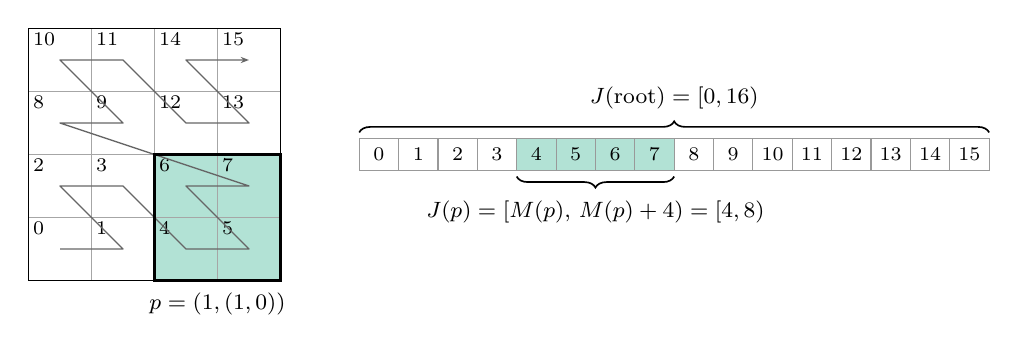
\begin{tikzpicture}
    \fill[r2!30] (1.6,0) rectangle (3.2,1.6);
    \foreach \k in {0,...,15} {
      \pgfmathtruncatemacro{\i}{mod(\k,2) + 2*mod(int(\k/4),2)}
      \pgfmathtruncatemacro{\j}{mod(int(\k/2),2) + 2*int(\k/8)}
      \draw[black!35] (\i*0.8,\j*0.8) rectangle ++(0.8,0.8);
      \node[font=\scriptsize, anchor=north west, inner sep=1.5pt]
        at (\i*0.8,\j*0.8+0.8) {\k};
    }
    \draw[black!60, line width=0.5pt, line join=round, -{Stealth[length=3pt]}]
      (0.4,0.4) -- (1.2,0.4) -- (0.4,1.2) -- (1.2,1.2) -- (2.0,0.4) --
      (2.8,0.4) -- (2.0,1.2) -- (2.8,1.2) -- (0.4,2.0) -- (1.2,2.0) --
      (0.4,2.8) -- (1.2,2.8) -- (2.0,2.0) -- (2.8,2.0) -- (2.0,2.8) --
      (2.8,2.8);
    \draw[black, line width=1.1pt] (1.6,0) rectangle (3.2,1.6);
    \draw[black, line width=0.6pt] (0,0) rectangle (3.2,3.2);
    \node[font=\footnotesize] at (2.4,-0.3) {$p = (1, (1,0))$};
    % the keys on a line
    \begin{scope}[xshift=4.2cm, yshift=1.4cm]
      \foreach \k in {0,...,15} {
        \pgfmathsetmacro{\c}{(\k >= 4 && \k < 8) ? 1 : 0}
        \ifdim \c pt > 0.5pt
          \filldraw[fill=r2!30, draw=black!40] (\k*0.5,0) rectangle ++(0.5,0.4);
        \else
          \draw[black!40] (\k*0.5,0) rectangle ++(0.5,0.4);
        \fi
        \node[font=\scriptsize] at (\k*0.5+0.25,0.2) {\k};
      }
      \draw[decorate, decoration={brace, amplitude=4pt, mirror},
        line width=0.6pt] (2.0,-0.08) -- (4.0,-0.08)
        node[midway, below=5pt, font=\footnotesize]
        {$J(p) = [M(p),\, M(p) + 4) = [4, 8)$};
      \draw[decorate, decoration={brace, amplitude=4pt},
        line width=0.6pt] (0,0.48) -- (8.0,0.48)
        node[midway, above=5pt, font=\footnotesize]
        {$J(\text{root}) = [0, 16)$};
    \end{scope}
  \end{tikzpicture}
  \caption{Keys of the finest cells ($D = 2$, $\ell_{\max} = 2$), written in
    each cell; the grey line is the Morton curve. The node $p$ (outlined)
    holds the keys 4 to 7, a stretch of the curve: its key interval.}
  \label{fig:keyint}
\end{figure}

Two facts follow and are used all through: a node $q$ lies inside $p$
exactly when $J(q) \subseteq J(p)$, and the owner of $p$ is decided by
where $M(p)$, the start of its stretch, falls among the cuts $K_r$
(definition~\ref{def:owner}).

\begin{proposition}[the curve]
  \label{prop:morton}
  For $p, q \in \mathcal{I}$:
  \begin{enumerate}[label=(\alph*)]
    \item $q \preceq p \iff J(q) \subseteq J(p)$, and two key intervals are
      nested or disjoint;
    \item $J(\chi_0(p)), \ldots, J(\chi_{2^D-1}(p))$ follow each other in
      this order and partition $J(p)$; so $M(p) = M(\chi_0(p))$, and a node
      has the key of its first leaf;
    \item for a tree $T$, $\{J(q)\}_{q \in \mathcal{L}}$ partitions $[0,
      2^{D \ell_{\max}})$: $M$ is injective on $\mathcal{L}$.
  \end{enumerate}
\end{proposition}

\begin{proof}
  The top $D\ell(p)$ bits of $M(p)$ are $Z$ of $\mathbf{i}(p)$ at level
  $\ell(p)$; the low $D(\ell_{\max} - \ell(p))$ bits are zero. A node below
  $p$ has the same top bits and any low bits, which is (a); bits $D(\ell_{
  \max} - \ell - 1)$ to $D(\ell_{\max} - \ell) - 1$ of a child's key are its
  $c$, which is (b). The leaf boxes partition $\Omega$, so the leaf
  intervals partition the finest keys: (c).
\end{proof}

$M$ is not injective on $T$ ($p$ and $\chi_0(p)$ share a key), but $(\ell,
M)$ is. The \emph{curve} is $\mathcal{L}$ sorted by key, $q_0, \ldots,
q_{N-1}$; $\sigma(q)$ is the position of $q$ on it (\fn{tree\_caches
()->leaves}).

% ----------------------------------------------------------------------
\subsection{Ranks, ownership, local sets}

\begin{definition}[ranks, weights]
  The ranks are $\mathcal{P} = \{0, 1, \ldots, n_{pe} - 1\}$. A weight is
  $w : \mathcal{L} \to \mathbb{R}_{>0}$; $W(q) = \sum_{\sigma(q') <
  \sigma(q)} w(q')$ is the weight before $q$ on the curve (the $W_q$ of
  section~\ref{sec:cut}), $W = \sum_{q} w(q)$ the total, $w_{\max} =
  \max_q w(q)$.
\end{definition}

\begin{definition}[partition table, ownership]
  \label{def:owner}
  A partition table is $K = (K_0, \ldots, K_{n_{pe}})$, $0 = K_0 \le K_1 \le
  \cdots \le K_{n_{pe}} = \infty$ (\fn{key\_first}). It defines the
  ownership map
  \[
    \rho = \rho_K : \mathcal{I} \to \mathcal{P}, \qquad
    \rho(p) = \max\{\, r \in \mathcal{P} : K_r \le M(p) \,\},
  \]
  the one $r$ with $K_r \le M(p) < K_{r+1}$ (so $K_r < K_{r+1}$: an empty
  rank owns nothing). $\rho$ is defined on every index, in $T$ or not,
  held here or not: a binary search, $O(\log n_{pe})$, no message
  (\fn{owner\_of\_key}, algorithm~\ref{alg:owner}). The pid a node stores
  is $\rho$ of it (\fn{node->pid}).
\end{definition}

\begin{definition}[local sets]
  \label{def:local}
  For $r \in \mathcal{P}$,
  \[
    \Lambda_r = \rho^{-1}(r) = \{p \in \mathcal{I} : K_r \le M(p) <
      K_{r+1}\}, \qquad
    T_r = T \cap \Lambda_r, \qquad
    \mathcal{L}_r = \mathcal{L} \cap \Lambda_r,
  \]
  the index piece, own nodes and own leaves of $r$ (\fn{tree\_caches
  ()->owned} is $\mathcal{L}_{me}$). The $\Lambda_r$ partition
  $\mathcal{I}$, so the $T_r$ partition $T$ and the $\mathcal{L}_r$
  partition $\mathcal{L}$. Each $\mathcal{L}_r$ is one run of the curve:
  $\sigma(\mathcal{L}_r)$ is an interval of integers. By
  proposition~\ref{prop:morton}(b) a node is owned by the owner of its
  first leaf. The load of $r$ is $\lambda_r = \sum_{q \in \mathcal{L}_r}
  w(q)$ and the imbalance $\eta = n_{pe} \max_r \lambda_r / W \ge 1$.
\end{definition}

\begin{definition}[valid table]
  \label{def:valid}
  $K$ is valid for $T$ when
  \begin{enumerate}[label=(V\arabic*)]
    \item each $K_r$ with $K_r < K_{r+1}$ is the key of a leaf (the first
      of $\mathcal{L}_r$);
    \item families of leaves are whole: if all children of $u \in T$ are
      leaves, $\rho$ is constant on them.
  \end{enumerate}
\end{definition}

\begin{proposition}[the cut]
  \label{prop:cut}
  Let $r(q) = \min\big(n_{pe} - 1, \lfloor n_{pe}(W(q) + w(q)/2)/W
  \rfloor\big)$ (section~\ref{sec:cut}), then $r(q) \gets r(\chi_0(\pi(q)))$
  for each $q$ in a family of leaves (algorithm~\ref{alg:family}). Then
  \begin{enumerate}[label=(\alph*)]
    \item $r$ is non-decreasing along the curve, and $K_s = \min\{M(q) :
      r(q) \ge s\}$ ($\min \emptyset = \infty$; \textsc{NewTable}) is a
      valid table with $\rho_K = r$ on $\mathcal{L}$;
    \item $\lambda_s \le W/n_{pe} + w_{\max}$ without the family rule, and
      $\lambda_s \le W/n_{pe} + 2^D w_{\max}$ with it.
  \end{enumerate}
\end{proposition}

\begin{proof}
  (a) $W(q) + w(q)/2$ grows along the curve, so the first $r$ does. A
  family of leaves is a run of the curve beginning with child~0
  (proposition~\ref{prop:morton}(b)); giving the whole run the value of
  its first element keeps a non-decreasing sequence non-decreasing. A
  non-decreasing $r$ cuts the curve into runs, and $K_s$ is the first key
  of run $s$ (or of the next non-empty one), which is (V1) and $\rho_K =
  r$; (V2) holds by construction. (b) The leaves of $s$ have their middles
  in $[sW/n_{pe}, (s+1)W/n_{pe})$, so they lie in that interval widened by
  $w_{\max}/2$ on each side. The family rule adds at most the $2^D - 1$
  siblings that follow the last child~0 of $s$.
\end{proof}

\begin{proposition}[adaptation keeps the table]
  \label{prop:adapt}
  Let $K$ be valid for $T$. If $T'$ is made from $T$ by dividing leaves,
  $K$ is valid for $T'$, and a new child has its parent's owner. If $T'$
  is made by merging families of leaves, (V1) still holds and the parent
  has its children's owner, but (V2) can fail.
\end{proposition}

\begin{proof}
  Let $p \in \mathcal{L}_r$. $K_{r+1}$ is $\infty$ or the key of a leaf $q
  \ne p$ with $M(q) > M(p)$; $J(q)$ and $J(p)$ are disjoint, so $K_{r+1} \ge
  \max J(p) + 1$ and $J(p) \subseteq [K_r, K_{r+1})$: every child of $p$ is
  in $\Lambda_r$. The children form a family of leaves on one rank: (V2).
  If $K_r = M(p)$, it is the key of $\chi_0(p)$ too: (V1). Merging: the
  children are on one rank by (V2), and the parent has child~0's key. If
  $K_r$ was a merged child's key, it was child~0's (a later sibling's key
  would come after child~0's, on the same rank), so it is the parent's.
  But the merge can make a new family of leaves, the parent and its
  siblings, whose members sit on different ranks (figure~\ref{fig:family}).
\end{proof}

So between two repartitions the table does not change: refining needs no
message about owners, and the next repartition puts back (V2).

% ----------------------------------------------------------------------
\subsection{Neighbourhood, halos, edge cut, communication graph}

\begin{definition}[neighbourhood]
  \label{def:nbhd}
  For $p \in T$ and $\delta \in \{-1, 0, 1\}^D \setminus \{\mathbf{0}\}$
  let $b_\delta = (\ell(p), \mathbf{i}(p) + \delta)$, taken only when it is
  in $\mathcal{I}$ (no periodicity). $N(p)$ is the set of
  \begin{itemize}
    \item $b_\delta$ when $b_\delta \in T$ (same level: ghosts);
    \item $\pi(b_\delta)$ when $b_\delta \notin T$ (a coarser leaf, by
      (T2) and (T4));
    \item when $p \in \mathcal{L}$ and $b_\delta \in T \setminus
      \mathcal{L}$: the children $\chi_c(b_\delta)$ that touch $p$,
      $\beta(c)_a = [\delta_a < 0]$ for each $a$ with $\delta_a \ne 0$
      (reflux, and the far side of a coarse neighbour);
    \item $\pi(p)$ and the children of $p$ (restriction).
  \end{itemize}
  This is \fn{related ()} in \fn{tree-mpi.c}. $N^*(p) = N(p) \cup \{p\}$
  and $N(S) = \bigcup_{p \in S} N(p)$.
\end{definition}

\begin{proposition}[symmetry]
  \label{prop:sym}
  For $p, x \in T$: $x \in N(p) \iff p \in N(x)$.
\end{proposition}

\begin{proof}
  Same level, and parent with child: symmetric as written. A coarse
  neighbour: $x = \pi(b_\delta)$ is a leaf one level above $p$, touching
  $p$. Seen from $x$, the node of its level across that side is $\pi(p)$
  ($\ne x$, since siblings come together), in $T$ with children, and $x$
  is a leaf; so $N(x)$ holds the children of $\pi(p)$ that touch $x$, $p$
  among them. A fine neighbour is the same case seen from the other side.
\end{proof}

\begin{definition}[graphs, edge cut]
  The node graph is $G_N = (T, E_N)$, $E_N = \{\{p, x\} : x \in N(p)\}$,
  undirected by proposition~\ref{prop:sym}. The leaf graph is $G_L =
  (\mathcal{L}, E_L)$, $E_L = \{\{p, q\} \subseteq \mathcal{L} : p \ne q,\
  \overline{\Omega(p)} \cap \overline{\Omega(q)} \ne \emptyset\}$, the graph
  usual in graph partitioning. The edge cut of $\rho$ is
  \[
    C(\rho) = \{\{p, x\} \in E_N : \rho(p) \ne \rho(x)\}, \qquad
    C_L(\rho) = \{\{p, q\} \in E_L : \rho(p) \ne \rho(q)\}.
  \]
  $C$ is what the plans exchange (ghosts, restriction, reflux); $C_L$
  counts only the ghosts of the leaves.
\end{definition}

\begin{definition}[halo]
  \label{def:halo}
  The halo of $r$ is the part of its neighbourhood it does not own, and
  its part from $s$:
  \[
    H_r = N(T_r) \setminus T_r = \{x : \{p, x\} \in C(\rho),\ \rho(p) = r,
      \ \rho(x) \ne r\}, \qquad
    H_r^s = H_r \cap \Lambda_s .
  \]
  $H_r \cap \mathcal{L}$ is the leaf halo (figure~\ref{fig:skeleton}).
\end{definition}

\begin{definition}[communication graph]
  \label{def:comm}
  $G_C = (\mathcal{P}, E_C)$, $E_C = \{\{r, s\} : r \ne s,\ H_r^s \ne
  \emptyset\}$: the image of $C(\rho)$ under $\rho \times \rho$, a quotient
  of $G_N$. The peers of $r$ are its neighbours in $G_C$, $Q_r = \rho(H_r)$.
  The edge $\{r, s\}$ carries $V_{rs} = |H_r^s|$ nodes from $s$ to $r$ and
  $V_{sr}$ back, in general $V_{rs} \ne V_{sr}$.
\end{definition}

By proposition~\ref{prop:sym}, $H_r^s \ne \emptyset \iff H_s^r \ne
\emptyset$: $s \in Q_r \iff r \in Q_s$. Each rank can therefore make its
receive lists alone and send them to its peers, who learn what to send
(algorithm~\ref{alg:skeleton}); there is no message to all ranks. Writing
$b$ for the bytes sent per node and $\alpha_{rs}$, $\beta_{rs}$ for the
latency and inverse bandwidth between $r$ and $s$ (what
\fn{mpi-topology.c} measures between nodes), one exchange takes about
\[
  t_{ex} \approx \max_{r \in \mathcal{P}} \sum_{s \in Q_r} \big(\alpha_{rs}
    + \beta_{rs}\, b\, V_{rs}\big).
\]
The degree $|Q_r|$ sets the latency term, the halo $|H_r|$ the volume.
The curve cut makes $\lambda_r$ even (proposition~\ref{prop:cut}) and
gives no bound on $|C(\rho)|$; it relies on a run of the curve being a
compact region (section~\ref{sec:problem}).

\begin{figure}[h]
  \centering
  \begin{subfigure}[b]{0.40\textwidth}
    \centering
    \begin{tikzpicture}[scale=0.62]\input{fig-family.tex}\end{tikzpicture}
    \caption{The partition $\rho$ of figure~\ref{fig:curve}b.}
  \end{subfigure}\hfill
  \begin{subfigure}[b]{0.28\textwidth}
    \centering
    \begin{tikzpicture}\input{fig-commgraph.tex}\end{tikzpicture}
    \caption{$G_C$; near $r$ on edge $\{r,s\}$: $V_{rs}$.}
  \end{subfigure}\hfill
  \begin{subfigure}[b]{0.28\textwidth}
    \centering\small
    \begin{tabular}{@{}lr@{}}
      \toprule
      $|\mathcal{L}|$ & \nleaves \\
      $|E_L|$ & \nedges \\
      $|C_L(\rho)|$ & \ncut \\
      $|E_C|$ & \ncommedges \\
      $|H_r \cap \mathcal{L}|$ & \halocounts \\
      $|Q_r|$ & \degrees \\
      \bottomrule
    \end{tabular}
    \caption{Measured on (a), $r = 0 \ldots 3$.}
  \end{subfigure}
  \caption{The edge cut and the communication graph of the example,
    computed by \fn{figures.py} on the leaf graph $G_L$ (leaves touching by
    a face or a corner), so $V_{rs}$ counts leaves of the halo. Rank~1's
    halo is the one of figure~\ref{fig:skeleton}. Ranks 0 and 3 touch
    nowhere: no edge.}
  \label{fig:comm}
\end{figure}

% ----------------------------------------------------------------------
\subsection{Ancestors and the skeleton}
\label{sec:skel-def}

\begin{definition}[skeleton]
  \label{def:skeleton}
  With $\mathrm{Fam}(S) = \bigcup_{p \in S} F(p)$, the skeleton of $r$ is
  \[
    S_r = \mathrm{Fam}\big(\bar A(T_r \cup N(T_r))\big) :
  \]
  own nodes, their neighbourhood, the ancestors of both, and the families
  of all of them (\fn{tree\_insert} adds missing ancestors with their
  families). $S_r$ satisfies (T1) to (T3). Its leaves that are not leaves
  of $T$ are the pruned nodes $\Pi_r = \mathcal{L}(S_r) \setminus
  \mathcal{L}$. The active nodes, with blocks, are $T_r \cup H_r$ (and the
  families with an active member); the rest of $S_r$ is inactive: flags
  and pid only.
\end{definition}

\begin{proposition}[ancestors of a piece]
  \label{prop:anc}
  $A(T_r) \setminus T_r \subseteq \{p \in T : M(p) < K_r < M(p) +
  |J(p)|\}$, which has at most one node on each level. So a rank holds at
  most $\ell_{\max}$ (in fact the depth of $T$) ancestors it does not own.
\end{proposition}

\begin{proof}
  Let $p$ be an ancestor of $q \in T_r$ with $p \notin \Lambda_r$. $J(q)
  \subseteq J(p)$, so $M(p) \le M(q) < K_{r+1}$, hence $M(p) < K_r \le M(q)
  < M(p) + |J(p)|$: $K_r$ is inside $J(p)$ and not its first key. The nodes
  of one level have disjoint intervals, and only one can hold $K_r$.
\end{proof}

The ancestors cost a rank a chain of nodes from the root down to its first
key, whatever $n_{pe}$ and the size of its piece. In
figure~\ref{fig:skeleton} the grey pruned nodes are most of what is held
beyond $T_r \cup H_r$.

% ----------------------------------------------------------------------
\subsection{Migration}

\begin{definition}[migration sets]
  Let $K^{old}$ and $K$ be the tables before and after a repartition,
  $\rho^{old}$ and $\rho$ their owners. For $r \ne s$,
  \[
    X_{r \to s} = \{p \in T : \rho^{old}(p) = r,\ \rho(p) = s\},
  \]
  what $r$ sends to $s$ (with $N(p)$, as structure, for each $p$:
  algorithm~\ref{alg:migrate}). The send and receive sets of $r$ are
  $\mathit{To}_r = \{s : X_{r \to s} \ne \emptyset\}$ and
  $\mathit{From}_r = \{o : X_{o \to r} \ne \emptyset\}$.
\end{definition}

\begin{proposition}[senders from the tables]
  \label{prop:from}
  If $K^{old}$ and $K$ satisfy (V1), then
  \[
    \mathit{From}_r = \{\, o \ne r : K^{old}_o < K^{old}_{o+1},\
      [K^{old}_o, K^{old}_{o+1}) \cap [K_r, K_{r+1}) \ne \emptyset \,\},
  \]
  a range of consecutive ranks from $\rho^{old}(K_r)$ to
  $\rho^{old}(K_{r+1} - 1)$ when the new piece of $r$ is not empty (empty
  ranks left out), known without a message.
  Every $o$ in it sends $r$ at least one leaf.
\end{proposition}

\begin{proof}
  $\subseteq$: a node sent from $o$ to $r$ has its key in both intervals.
  $\supseteq$: the left end of the intersection is $K^{old}_o$ or $K_r$,
  by (V1) the key of a leaf, and that leaf is in both pieces: $o$ owned it,
  $r$ owns it now. The intersection with $[K_r, K_{r+1})$ of a partition
  of the keys into consecutive intervals is a run of consecutive intervals.
\end{proof}

So \textsc{Exchange} (algorithm~\ref{alg:exch}) never waits for a message
nobody sends. One pass sends each node whose owner changes exactly once,
$\sum_{r \ne s} |X_{r \to s}|$ nodes in all, which is the least possible.
Moves to rank $\pm 1$ (Basilisk, figure~\ref{fig:iterate}) carry $p$ at
least $|\rho(p) - \rho^{old}(p)|$ times and take at least $\max_p |\rho(p)
- \rho^{old}(p)|$ passes.

% ----------------------------------------------------------------------
\subsection{AMR with MPI}
\label{sec:amr-mpi}

\begin{definition}[distributed state]
  \label{def:state}
  A distributed AMR state is $\mathfrak{S} = \big(T, K, (S_r, u_r)_{r \in
  \mathcal{P}}\big)$, where $u_r$ gives each active node of $S_r$ its
  blocks, one per scalar. It satisfies
  \begin{enumerate}[label=(I\arabic*)]
    \item $T$ is a tree: (T1) to (T4);
    \item $K$ is valid for $T$: (V1) always, (V2) after each step (a merge
      that breaks it forces a repartition);
    \item rank $r$ holds exactly $S_r$, and the pid of each node of $S_r$ is
      $\rho_K$ of it; every $K$ is on every rank;
    \item $u_r(p)$ is the value of $p$ for $p \in T_r$; for $x \in H_r$,
      $u_r(x)$ is a copy, current when $u_r(x) = u_{\rho(x)}(x)$.
  \end{enumerate}
  Nothing of $T \setminus \bigcup_r S_r$ is held anywhere, and no rank
  stores anything of size $|T|$; only $K$ has size $n_{pe}$.
\end{definition}

A step of a simulation is a composition of four operations on
$\mathfrak{S}$:
\begin{description}[leftmargin=1.4em, font=\normalfont\itshape]
  \item[Exchange $E$] (\fn{ghosts\_update}, \fn{ghosts\_update\_levels}):
    $u_r(x) \gets u_{\rho(x)}(x)$ for $x \in H_r$, or for the part a plan
    names (ghosts, restriction, faces; by level). Messages go only along
    the edges of $G_C$, both ways.
  \item[Compute $F$]: $u_r(p) \gets f\big(u_r|_{N^*(p)}\big)$ for each $p
    \in T_r$.
  \item[Adapt $A$] (\fn{tree\_mpi\_refine}, coarsening): $T \to T'$, own
    leaves divided or merged, the 2:1 closure across ranks by rounds
    between peers; $K$ unchanged (proposition~\ref{prop:adapt}); $S_r$ and
    $H_r$ made again.
  \item[Repartition $R$] (\fn{tree\_mpi\_repartition}): new $K$ by
    proposition~\ref{prop:cut}, migration by proposition~\ref{prop:from},
    then $S_r$, $Q_r$ and the plans (algorithm~\ref{alg:skeleton}).
\end{description}
\[
  \mathfrak{S}^{n+1} = \begin{cases}
    R \circ A \circ F \circ E\,(\mathfrak{S}^n) & \text{if, after } A,
      \text{ (V2) fails or } \max_r |\mathcal{L}_r| > \max\big(
      \eta_{\max} N/n_{pe},\, \lceil N/n_{pe} \rceil + 2^D - 1\big),\\
    A \circ F \circ E\,(\mathfrak{S}^n) & \text{otherwise}
  \end{cases}
\]
(unit weights, \fn{adapt\_wavelet ()}: section~\ref{sec:when},
algorithm~\ref{alg:when}).

\begin{proposition}[the same as on one rank]
  \label{prop:serial}
  Let $f$ read, for a node $p$, only nodes of $N^*(p)$. After $E$, $F$ on
  the distributed state gives on every $p \in T_r$ the value that $F$ on
  the whole tree $T$ held by one process gives.
\end{proposition}

\begin{proof}
  $N^*(p) \subseteq T_r \cup H_r$ for $p \in T_r$, by
  definition~\ref{def:halo}. After $E$ every value there equals the
  owner's (I4), which is the one-process value by induction on the steps.
\end{proof}

With $\mathrm{GHOSTS} = 2 \le m$, a stencil of radius 2 about any cell of
$p$'s block stays in the boxes of $N^*(p)$, so the solvers' stencils meet
the condition. The tests compare the distributed fields with the
one-process ones bit for bit.

\begin{table}[h]
  \centering\small
  \begin{tabular}{@{}l l l@{}}
    \toprule
    symbol & meaning & in the code \\
    \midrule
    $\mathcal{I}$, $p = (\ell, \mathbf{i})$ & indices & \fn{Index} \\
    $\pi$, $\chi_c$, $F$ & parent, child $c$, family & \fn{index\_parent},
      \fn{index\_child} \\
    $A$, $\bar A$ & ancestors, with the set itself & \\
    $T$, $\mathcal{L}$ & the whole tree, its leaves & \\
    $M$, $J(p)$ & Morton key, key interval & \fn{tree\_morton\_key} \\
    $\sigma$ & position on the curve & \fn{tree\_caches ()->leaves} \\
    $\mathcal{P}$, $n_{pe}$, $me$ & ranks, their number, this one &
      \fn{tree\_npe}, \fn{tree\_rank} \\
    $w$, $W(q)$, $W$ & weights, weight before $q$, total & \fn{weight} \\
    $K$ & partition table & \fn{key\_first} \\
    $\rho = \rho_K$ & ownership $\mathcal{I} \to \mathcal{P}$ &
      \fn{owner\_of\_key}, \fn{node->pid} \\
    $\Lambda_r$, $T_r$, $\mathcal{L}_r$ & index piece, own nodes, own leaves
      & \fn{tree\_caches ()->owned} \\
    $\lambda_r$, $\eta$ & load, imbalance & \\
    $N(p)$, $N^*(p)$ & neighbourhood, with $p$ & \fn{related} \\
    $E_N$, $E_L$ & node graph, leaf graph & \\
    $C(\rho)$, $C_L(\rho)$ & edge cuts & \\
    $H_r$, $H_r^s$ & halo, its part from $s$ & the receive lists \\
    $G_C$, $Q_r$, $V_{rs}$ & communication graph, peers, volume &
      \fn{TreeMpiPlan} \\
    $S_r$, $\Pi_r$ & skeleton, pruned nodes & \fn{skeleton\_and\_plan} \\
    $X_{r\to s}$ & migration set & \textsc{Migrate} \\
    $\mathfrak{S}$ & distributed state & \\
    \bottomrule
  \end{tabular}
  \caption{The notation of section~\ref{sec:defs}.}
  \label{tab:notation}
\end{table}


% ======================================================================
\section{The cut: prefix sums along the curve}
\label{sec:cut}

Let $w_q$ be the weight of leaf $q$ in curve order, $W_q = \sum_{p<q} w_p$
the weight before it and $W$ the total. Leaf $q$ goes to rank
\[
  r(q) \;=\; \min\!\Big(n_{pe}-1,\;
    \Big\lfloor n_{pe}\,\frac{W_q + w_q/2}{W} \Big\rfloor\Big),
\]
the rank whose share $[\,rW/n_{pe},\,(r+1)W/n_{pe})$ holds the leaf's
middle. Figure~\ref{fig:weights} draws it.

\begin{figure}[h]
  \centering
  \begin{tikzpicture}\input{fig-weights.tex}\end{tikzpicture}
  \caption{Twenty leaves with weights 1 to 4 (width and number), $W =
    \wtotal$, 4 ranks. The dashed lines are the ideal cuts at $kW/4$; a
    dot is a leaf's middle, and the leaf's colour is the share the dot
    falls in. The small numbers below are the prefix sums $W_q$.}
  \label{fig:weights}
\end{figure}

\textbf{On a distributed tree} no rank sees all the weights, and each
rank's own leaves are one contiguous run of the curve. Two collectives of
a few doubles per rank give it all it needs:
\begin{itemize}
  \item \fn{MPI\_Allreduce} of (count, weight, bad), bad counting the
    weights not $> 0$: the totals $N$ and $W$, and whether to stop
    (on every rank, nothing changed);
  \item \fn{MPI\_Exscan} of (count, weight): the leaves and the weight
    before my first leaf.
\end{itemize}
Counts travel as doubles, exact below $2^{53}$. The weight check and the
two totals used to be three \fn{MPI\_Allreduce}s and the two prefixes two
\fn{MPI\_Exscan}s; each collective costs at least $\lceil\log_2
n_{pe}\rceil$ message latencies (section~\ref{sec:collectives}), so the
values go together.
Every rank then applies the formula to its own leaves alone. With integer
weights the answer is bit for bit the one a single rank holding the whole
tree would give (\fn{tree\_partition ()}); with fractional weights a leaf
on a tie may fall the other way, since the sums are added in another
order.

\textbf{How good is it?} Cutting a weighted sequence into $n_{pe}$
contiguous pieces with the smallest largest piece is the
\emph{chain-on-chains} problem \cite{pinar}. The prefix rule is within one
leaf's weight of the optimum; \fn{test\_partition} checks this against
the optimum found by bisection on the bound with greedy packing.

\subsection{The new table, without a reduction}
\label{sec:table}

After the cut every rank must know the whole new table $K$ (the first key
of every rank, definition~\ref{def:owner}), and with it each rank's leaves
and load. No rank needs to \emph{add} anything up for it: since $r$ does
not decrease along the curve (proposition~\ref{prop:cut}(a)),
\[
  K_s = \min\{M(q) : r(q) \ge s\}
\]
is the key of one leaf, the first with $r(q) \ge s$, and the one rank
holding that leaf also knows its prefix weight $W(q)$ and its index along
the curve (from the \fn{MPI\_Exscan}). That rank gives the entry
$(K_s, W(K_s), n(K_s))$, 24 bytes; the others give nothing for $s$.

Which rank gives which entries? Let rank $o$ hold leaves whose ranks end
with $r_{last}(o)$ ($-1$ if it holds none), and let $\ell_o = \max_{o' <
o} r_{last}(o')$ ($-1$ for $o = 0$). Rank $o$ gives the entries
\[
  s = \ell_o + 1, \ldots, r_{last}(o), \qquad c_o = \max\big(0,\;
    r_{last}(o) - \ell_o\big) \text{ of them}.
\]

\begin{proposition}[one giver per entry]
  \label{prop:giver}
  The ranges $(\ell_o, r_{last}(o)]$ are disjoint, their union is
  $[0, r_{\max}]$ with $r_{\max}$ the rank of the last leaf, and the first
  leaf with $r(q) \ge s$, for $s$ in the range of $o$, is a leaf of $o$.
\end{proposition}

\begin{proof}
  $\ell_{o+1} = \max(\ell_o, r_{last}(o))$, so the ranges follow each
  other without overlap and, by telescoping, cover $[0, r_{\max}]$. For
  $s \in (\ell_o, r_{last}(o)]$: the leaves of the ranks before $o$ have
  $r \le \ell_o < s$, and $o$ has a leaf with $r = r_{last}(o) \ge s$;
  the ranks own consecutive runs of the curve, so the first leaf with $r
  \ge s$ is one of $o$'s.
\end{proof}

So the table takes two collectives, both without a reduction:
\begin{enumerate}
  \item \fn{MPI\_Allgather} of $r_{last}$, one int a rank: every rank
    computes every $c_o$ and the displacements;
  \item \fn{MPI\_Allgatherv} of the entries: they arrive in the order of
    $s$, $\sum_o c_o = r_{\max} + 1 \le n_{pe}$ of them.
\end{enumerate}
Then $K_s$, $W(K_s)$ and $n(K_s)$ for $s > r_{\max}$ are $\infty$, $W$
and $N$ (empty ranks at the end); $K_0 = 0$; the load of $s$ is
$\lambda_s = W(K_{s+1}) - W(K_s)$ and its first leaf
\fn{leaf\_first}$[s] = n(K_s)$. An empty rank in the middle gets the key
of the next non-empty one, as before, because its first leaf with $r \ge
s$ is that one's. Keys and counts are exact; with fractional weights a
load, a difference of two prefix sums, may differ in the last bits from
the sum of the leaves' weights (it only feeds the imbalance).

\begin{figure}[h]
  \centering
  \begin{tikzpicture}[x=1cm, y=1cm]\input{fig-entries.tex}\end{tikzpicture}
  \caption{Who gives the entries of the new table. The colours are the new
    ranks, the black frames the old pieces, the number under a frame the
    entries that old rank gives. Top: the example of
    figure~\ref{fig:onepass} (rank 0 refined twice): old rank 0 holds the
    first leaf of every new piece and gives all four entries (counts
    \entbig). Bottom: a small change (one leaf more on rank 2 after the
    one pass): each rank gives one entry (counts \entsmall), the usual
    case after a step.}
  \label{fig:entries}
\end{figure}

Before, the table was one \fn{MPI\_Allreduce} of $n_{pe}$ entries
$\{$smallest key, load, count$\}$ with a user operation (key the
smaller, load and count summed): every rank filled $n_{pe}$ entries, all
but one or two the identity, and the reduction combined them all.
Section~\ref{sec:collectives} compares the two.

% ======================================================================
\section{Families stay whole}

Coarsening merges a family of $2^D$ sibling leaves into their parent. If
the siblings sit on different ranks, the merge needs their data in one
place first. libb-amr never splits a family of leaves: after the middle
rule, each such family goes to the rank of its child~0, the first sibling
along the curve (figure~\ref{fig:curve}b). The cost is a small imbalance,
less than one family per cut.

\begin{figure}[h]
  \centering
  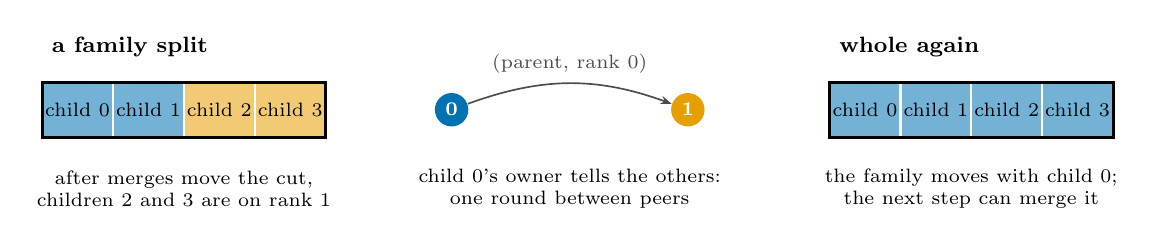
\begin{tikzpicture}[x=1cm, y=1cm]
    % before: a family split by a merge elsewhere
    \begin{scope}
      \node[font=\footnotesize\bfseries, anchor=west] at (0,2.35)
        {a family split};
      \foreach \c/\k in {0/0, 1/0, 2/1, 3/1}
        \filldraw[fill=r\k!55, draw=white, line width=0.8pt]
          (\c*0.9, 1.2) rectangle ++(0.9, 0.7);
      \foreach \c in {0,1,2,3}
        \node[font=\scriptsize] at (\c*0.9+0.45, 1.55) {child \c};
      \draw[black, line width=1.1pt] (0,1.2) rectangle (3.6,1.9);
      \node[font=\scriptsize, align=center] at (1.8,0.55)
        {after merges move the cut,\\children 2 and 3 are on rank 1};
    \end{scope}
    % the message
    \begin{scope}[xshift=5.2cm]
      \node[circle, fill=r0, text=white, font=\scriptsize\bfseries,
        inner sep=2pt] (a) at (0,1.55) {0};
      \node[circle, fill=r1, text=white, font=\scriptsize\bfseries,
        inner sep=2pt] (b) at (3.0,1.55) {1};
      \draw[flow] (a) to[bend left=20]
        node[above, font=\scriptsize, align=center]
          {(parent, rank 0)} (b);
      \node[font=\scriptsize, align=center] at (1.5,0.55)
        {child 0's owner tells the others:\\one round between peers};
    \end{scope}
    % after
    \begin{scope}[xshift=10.0cm]
      \node[font=\footnotesize\bfseries, anchor=west] at (0,2.35)
        {whole again};
      \foreach \c in {0,1,2,3}
        \filldraw[fill=r0!55, draw=white, line width=0.8pt]
          (\c*0.9, 1.2) rectangle ++(0.9, 0.7);
      \foreach \c in {0,1,2,3}
        \node[font=\scriptsize] at (\c*0.9+0.45, 1.55) {child \c};
      \draw[black, line width=1.1pt] (0,1.2) rectangle (3.6,1.9);
      \node[font=\scriptsize, align=center] at (1.8,0.55)
        {the family moves with child 0;\\the next step can merge it};
    \end{scope}
  \end{tikzpicture}
  \caption{When child~0 is mine, my following siblings take my rank
    without a message. A family split by earlier merges is settled by one
    message from child~0's owner to the other owners; siblings are in each
    other's neighbourhood $N()$, so their owners are always peers.}
  \label{fig:family}
\end{figure}

p4est reaches the same goal differently: \fn{p4est\_partition\_for\_%
coarsening ()} shifts the piece boundaries while it computes the cut
\cite{p4est}. In the two Basilisk files read for this note
(\fn{balance.h}, \fn{tree-mpi.h}) no such rule was found.

% ======================================================================
\section{When to repartition}
\label{sec:when}

A repartition costs its collectives, the migration and a second rebuild of
the skeleton and plan (\fn{adapt\_wavelet ()} has just made one). After a
small adaptation the old cut is often still as good as a new one, so
\fn{adapt\_wavelet ()} repartitions only when it must. Its last step is
one \fn{MPI\_Allreduce} of five numbers (a user operation: the first three
summed, the last two the larger): the leaves divided and the families
merged (the counts it returns), $N$, $\max_r |\mathcal{L}_r|$, and a flag,
1 where a family of leaves has a member on another rank. Then, with unit
weights and $\eta_{\max}$ = \fn{tree\_mpi\_imbalance\_max} (1 by
default),
\[
  \text{repartition} \iff \text{a family of leaves is split}
  \;\;\text{or}\;\; \max_r |\mathcal{L}_r| > \max\Big(\eta_{\max}
  \frac{N}{n_{pe}},\; \Big\lceil \frac{N}{n_{pe}} \Big\rceil + 2^D -
  1\Big).
\]

\begin{proposition}[what a cut leaves, unit weights]
  \label{prop:unitcut}
  With $w \equiv 1$, the cut of proposition~\ref{prop:cut} leaves every
  rank at most $\lceil N/n_{pe} \rceil + 2^D - 1$ leaves.
\end{proposition}

\begin{proof}
  The middle rule gives rank $s$ the leaves $g$ (their index along the
  curve) with $s \le n_{pe}(2g+1)/(2N) < s+1$, that is $sN/n_{pe} - 1/2
  \le g < (s+1)N/n_{pe} - 1/2$: an interval of length $N/n_{pe}$, so at
  most $\lceil N/n_{pe} \rceil$ integers. The family rule moves a boundary
  only later, past the siblings that follow a child~0, at most $2^D - 1$
  leaves, and a boundary meets at most one family. Rank $s$ loses at its
  start and gains at most $2^D - 1$ at its end.
\end{proof}

So with $\eta_{\max} = 1$ a partition is kept as long as no rank has more
leaves than a fresh cut could leave it; with $\eta_{\max} = 1.2$, until
some rank is 20\,\% above the mean. Only the largest piece is tested: an
underloaded rank does not slow the step.

\textbf{Why a split family forces it.} Coarsening merges a family only on
its parent's owner, and only if every child is a leaf of that owner,
flagged there (\fn{tree\_mpi\_coarsen ()}: a family is never split). A
merge can leave a family of leaves across two ranks
(figure~\ref{fig:family}, left). Kept so, the family could not merge at
the next adaptation, though the one-process tree would merge it, and the
distributed tree would no longer be the one-process tree. The flag sends
it to the cut, whose family rule makes it whole again
(\fn{test\_adapt\_mpi}: a cut set by weights between a divided leaf and
its siblings, then two coarsenings; with the flag ignored the second
merge is missed and the cells differ).

\textbf{What a kept partition still gives.} $K$ stays valid: (V1) by
proposition~\ref{prop:adapt}, (V2) by the flag, so every pid is still
$\rho_K$ of its node and \fn{tree\_partition\_owner ()} still names the
owner of any index; the state of section~\ref{sec:amr-mpi} holds. The
partition's loads, \fn{leaf\_first} and imbalance describe the tree of the
last repartition, and \fn{tree\_partition\_valid ()} turns 0 on the ranks
whose tree changed.

% ======================================================================
\section{Moving the nodes}

After adaptation the old pieces are out of balance. Two ways to reach the
new cut are drawn below on one example: 4 ranks of 4 leaves each, then
rank~0 refines its 4 leaves twice, giving \mleaves{} leaves, 64 of them on
rank~0.

\subsection{One pass, to the final rank (libb-amr, p4est)}

Every rank computes the new rank of each of its nodes (section
\ref{sec:cut}) and sends each node straight there. A rank knows whom it
receives from too: the old owners of its new piece, a contiguous range of
ranks found in the old table of first keys.

\begin{figure}[h]
  \centering
  \begin{tikzpicture}\input{fig-onepass.tex}\end{tikzpicture}
  \caption{One pass. Top: the owners after adapting; bottom: the owners
    after the move. The numbers in the bars are the leaves per rank. The
    graph on the right is who sends how many leaves to whom:
    \movedonce{} leaves move once, in one round of \pairsonce{} messages,
    some over three ranks (0 to 3).}
  \label{fig:onepass}
\end{figure}

\subsection{Moves of one rank, repeated (Basilisk)}

Basilisk's \fn{balance ()} computes each cell's target the same way (from
the weight before the cell), then clamps it to the cell's rank $\pm 1$:
\fn{pid = clamp (pid, cell.pid - 1, cell.pid + 1)}. Cells go only to
\fn{pid () - 1} and \fn{pid () + 1}, and \fn{mpi\_boundary\_update ()}
repeats \fn{while (balance (balance\_weights));} until no rank changes
anything (one \fn{mpi\_all\_reduce} of a flag).

\begin{figure}[h]
  \centering
  \begin{tikzpicture}\input{fig-iterate.tex}\end{tikzpicture}
  \caption{The same example, moves of one rank. \npasses{} passes, then a
    fourth finds nothing to do. The leaves that end three ranks away
    travel through ranks 1 and 2: \moveditr{} moves in all, against
    \movedonce{} in one pass, and the halo lists are rebuilt after every
    pass. Each pass talks only to the two neighbours on the curve. (The
    target here is taken from a leaf's start, as Basilisk does, so the
    final counts differ by one from figure~\ref{fig:onepass}.)}
  \label{fig:iterate}
\end{figure}

\textbf{The trade.} A pass to $\pm 1$ needs no table of where pieces
start: the two partners are fixed. But a shift of $k$ ranks takes $k$
passes, and every pass carries data and rebuilds the halo. After a small
change (the usual case, each step) both methods take one pass; after a
large one, as a first refinement on one rank or a front crossing the
domain, the single pass wins.

% ======================================================================
\section{The weight before a cell, without a collective}

libb-amr gets $W_q$ from \fn{MPI\_Exscan}. Basilisk's \fn{z\_weights ()}
gets it from the tree itself, with the halo exchanges it already has:
\begin{enumerate}
  \item bottom up, level by level: each node's subtree weight is the sum
    of its children's (\fn{boundary\_iterate (restriction, ...)});
  \item top down: child~$c$'s offset is its parent's plus the subtree
    weights of children $0 \ldots c-1$.
\end{enumerate}
Only the total is a collective: rank~0 has it at the root and shares it
with one \fn{mpi\_all\_reduce}.

\begin{figure}[h]
  \centering
  \begin{subfigure}[t]{0.48\textwidth}
    \centering
    \begin{tikzpicture}\input{fig-zup.tex}\end{tikzpicture}
    \caption{Up: subtree weights (each leaf 1).}
  \end{subfigure}\hfill
  \begin{subfigure}[t]{0.48\textwidth}
    \centering
    \begin{tikzpicture}\input{fig-zdown.tex}\end{tikzpicture}
    \caption{Down: the weight before each node; a leaf's is its $W_q$.}
  \end{subfigure}
  \caption{The two sweeps on a binary tree (the 1D case) of \zleaves{}
    leaves. The leaves are coloured by the rank they go to on 4 ranks,
    $\lfloor 4\,W_q / W \rfloor$. Each sweep costs one exchange per level,
    so about twice the depth in rounds, all between neighbours.}
  \label{fig:zweights}
\end{figure}

% ======================================================================
\section{Who owns a node?}

A rank must name the owner of a neighbour (for the halo) and, after a
move, the new owner of every node it keeps. Three ways:

\begin{figure}[h]
  \centering
  \begin{subfigure}[t]{\textwidth}
    \centering
    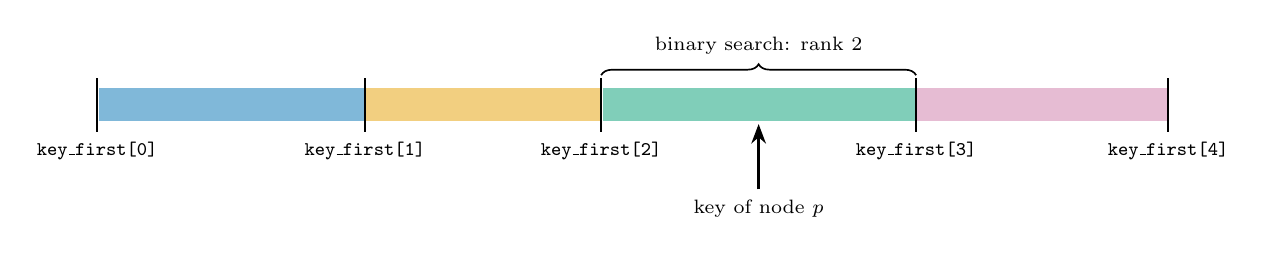
\begin{tikzpicture}[x=1cm, y=1cm]
      \foreach \k/\a/\b in {0/0/3.4, 1/3.4/6.4, 2/6.4/10.4, 3/10.4/13.6}
        \filldraw[fill=r\k!50, draw=white, line width=1pt]
          (\a,0) rectangle (\b,0.45);
      \foreach \k/\x in {0/0, 1/3.4, 2/6.4, 3/10.4, 4/13.6} {
        \draw[line width=0.7pt] (\x,-0.12) -- (\x,0.57);
        \node[font=\scriptsize, below] at (\x,-0.12)
          {\fn{key\_first[\k]}};
      }
      \draw[-{Stealth}, line width=0.9pt] (8.4,-0.85) node[below,
        font=\scriptsize] {key of node $p$} -- (8.4,-0.02);
      \draw[decorate, decoration={brace, amplitude=4pt}, line width=0.6pt]
        (6.4,0.6) -- (10.4,0.6) node[midway, above=4pt, font=\scriptsize]
        {binary search: rank 2};
    \end{tikzpicture}
    \caption{A table of first keys (libb-amr): $n_{pe}+1$ keys on every
      rank, $8\,n_{pe}$ bytes. The owner of \emph{any} index is a binary
      search, $O(\log n_{pe})$, with no message. Kept old and new across a
      move, it gives each rank its senders and receivers.}
  \end{subfigure}

  \vspace{4mm}
  \begin{subfigure}[t]{0.42\textwidth}
    \centering
    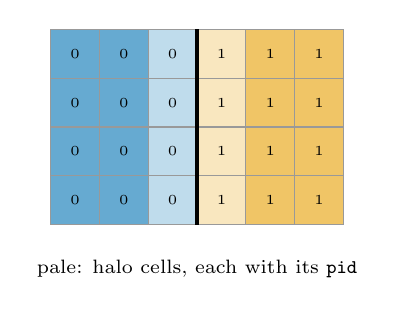
\begin{tikzpicture}[x=0.62cm, y=0.62cm]
      \foreach \i in {0,...,5} \foreach \j in {0,...,3} {
        \pgfmathtruncatemacro{\k}{\i<3 ? 0 : 1}
        \pgfmathtruncatemacro{\h}{(\i==2 || \i==3) ? 1 : 0}
        \ifnum\h=1
          \filldraw[fill=r\k!25, draw=black!40] (\i,\j) rectangle ++(1,1);
        \else
          \filldraw[fill=r\k!60, draw=black!40] (\i,\j) rectangle ++(1,1);
        \fi
        \node[font=\tiny] at (\i+0.5,\j+0.5) {\k};
      }
      \draw[line width=1.2pt] (3,0) -- (3,4);
      \node[font=\scriptsize, align=center] at (3,-0.9)
        {pale: halo cells, each with its \fn{pid}};
    \end{tikzpicture}
    \caption{A pid on every cell the rank holds, its own and its halo
      (Basilisk's \fn{cell.pid}, libb-amr's \fn{node->pid}). Enough for
      neighbours, nothing beyond them. After a move the sender tells the
      receiving neighbour the new pids.}
  \end{subfigure}\hfill
  \begin{subfigure}[t]{0.54\textwidth}
    \centering
    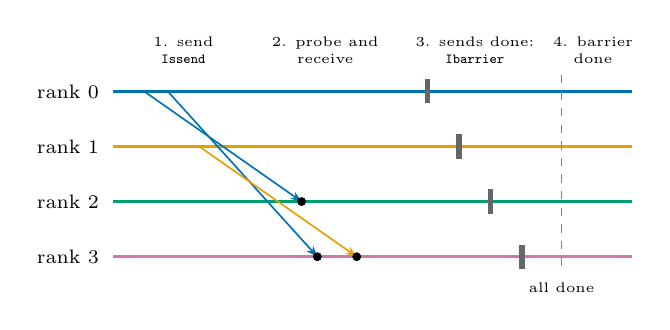
\begin{tikzpicture}[x=1cm, y=0.7cm]
      \foreach \k in {0,...,3} {
        \draw[r\k, line width=1pt] (0,-\k) -- (6.6,-\k);
        \node[anchor=east, font=\scriptsize] at (-0.05,-\k) {rank \k};
      }
      % phase labels
      \node[font=\tiny, align=center] at (0.9,0.75) {1. send\\\fn{Issend}};
      \node[font=\tiny, align=center] at (2.7,0.75) {2. probe and\\receive};
      \node[font=\tiny, align=center] at (4.6,0.75) {3. sends done:\\\fn{Ibarrier}};
      \node[font=\tiny, align=center] at (6.1,0.75) {4. barrier\\done};
      % sends: 0 -> 2, 0 -> 3, 1 -> 3
      \draw[flow, r0] (0.4,0) -- (2.4,-2);
      \draw[flow, r0] (0.7,0) -- (2.6,-3);
      \draw[flow, r1] (1.1,-1) -- (3.1,-3);
      % receives
      \foreach \k/\x in {2/2.4, 3/2.6, 3/3.1}
        \fill[black] (\x,-\k) circle (1.6pt);
      % barrier entries: after own sends are matched
      \foreach \k/\x in {0/4.0, 1/4.4, 2/4.8, 3/5.2}
        \draw[line width=2pt, black!60] (\x,-\k+0.22) -- (\x,-\k-0.22);
      \draw[dashed, black!50] (5.7,0.3) -- (5.7,-3.3);
      \node[font=\tiny, anchor=north] at (5.7,-3.3) {all done};
    \end{tikzpicture}
    \caption{No table, with NBX \cite{nbx}: the receivers need not know
      their senders. Each rank sends with synchronous sends, receives
      whatever arrives, and enters a non-blocking barrier once its own
      sends are matched; when the barrier completes, nothing is left in
      flight. Cost: a barrier, $O(\log n_{pe})$, instead of the table.}
  \end{subfigure}
  \caption{Finding owners. libb-amr uses (a) and (b) together: the table
    for any node after a move, the pid per node for the halo. Basilisk
    uses (b) only, which is why it moves cells only to $\pm 1$.}
  \label{fig:owners}
\end{figure}

\textbf{Arrays of size $n_{pe}$.} Outside a debugging check
(\fn{check\_snd\_rcv\_matrix ()}), Basilisk keeps none: its send and
receive lists (\fn{RcvPid}, one \fn{Rcv} per neighbouring rank and level)
are sized by the neighbours. In libb-amr the table is kept (\fn{key\_first},
\fn{leaf\_first}, \fn{load}: $20\,(n_{pe}+1)$ bytes), and the repartition
gathers it with \fn{MPI\_Allgather} of an int a rank and
\fn{MPI\_Allgatherv} of $n_{pe}$ entries of 24 bytes
(section~\ref{sec:table}): $O(n_{pe})$ received, the least a rank can
receive to hold the whole table. To drop the table too: (c) for the
senders and receivers of a move, and a round in which senders tell their
peers the new pids, plus one forwarding round for a node moved by a third
rank; \fn{tree\_partition\_owner ()} would then answer only on the
skeleton.

% ======================================================================
\section{What a rank keeps: the skeleton}
\label{sec:skeleton}

No rank holds the whole tree. libb-amr keeps the \emph{skeleton}: its own
nodes, their ancestors, and the neighbourhood $N(p)$ of each own node $p$
(the same-level neighbours, the coarse leaf covering an absent one, the
touching children of a neighbour with children, $p$'s parent and
children). The ranks owning $N()$ are the peers; the relation is
symmetric, so every exchange is between peers. Below $N()$ a node is
\emph{pruned}: it is kept, but its children are not.

\begin{figure}[h]
  \centering
  \begin{tikzpicture}
    \input{fig-skeleton.tex}
    \begin{scope}[xshift=6.6cm, yshift=4.6cm,
        every node/.style={font=\footnotesize, anchor=west}]
      \filldraw[fill=r1!70, draw=black!50] (0,0) rectangle (0.4,0.3);
      \node at (0.5,0.15) {own leaves of rank 1 (\nown)};
      \filldraw[fill=r0!38, draw=r0!80!black] (0,-0.6) rectangle (0.4,-0.3);
      \filldraw[fill=r2!38, draw=r2!80!black] (0.2,-0.6) rectangle (0.4,-0.3);
      \node at (0.5,-0.45) {halo: leaves touching them (\nhalo),};
      \node at (0.5,-0.85) {in their owner's colour};
      \filldraw[fill=black!12, draw=black!55] (0,-1.45) rectangle (0.4,-1.15);
      \node at (0.5,-1.3) {pruned nodes (\npruned): kept, no children};
      \node[align=left] at (0,-2.3)
        {\nskel{} nodes held in all: own, halo,\\ancestors and pruned};
    \end{scope}
  \end{tikzpicture}
  \caption{The tree of figure~\ref{fig:curve}b seen from rank 1.
    Simplified: $N(p)$ is drawn as the leaves touching $p$ (by a face or a
    corner); the real rule adds the neighbours of own parents. Halo nodes
    received with data have blocks; a family has blocks iff it has an
    active member. Basilisk's equivalent: local cells, the halo, and the
    needed ancestors, unused halo cells coarsened away.}
  \label{fig:skeleton}
\end{figure}

% ======================================================================
\clearpage
\section{Collectives: algorithms and costs}
\label{sec:collectives}

\subsection{The cost model}

A message of $b$ bytes between two ranks costs $\alpha + b\beta$: a
latency $\alpha$ (about 1\,\textmu s between nodes, 0.2 to 1\,\textmu s
within one) and a time per byte $\beta$ (0.1\,ns at 10\,GB/s). Combining
$b$ bytes in a reduction costs $b\gamma$. A rank sends and receives one
message at a time, both at once \cite{chan, thakur}. Two lower bounds hold
for any algorithm on $p$ ranks in which every rank's result depends on
every rank's input (\fn{MPI\_Allreduce}, \fn{MPI\_Allgather}):
\begin{itemize}
  \item \textbf{latency} $\lceil\log_2 p\rceil\,\alpha$: in a round, the
    ranks that know a given input can at most double;
  \item \textbf{bandwidth}: an allgather of $N$ bytes in all, $m = N/p$
    from each rank, makes every rank receive $(p-1)m$ bytes:
    $\frac{p-1}{p}N\beta$; an allreduce of $n$ bytes needs
    $2\frac{p-1}{p}n\beta$ \cite{patarasuk} and $\frac{p-1}{p}n\gamma$
    (each result byte is combined from $p$ inputs, the work shared by $p$
    ranks).
\end{itemize}

\subsection{Allreduce}

Three algorithms cover most of what MPI libraries choose from. Open MPI
4.1.6 offers basic linear, nonoverlapping, recursive doubling, ring,
segmented ring and Rabenseifner (as \fn{ompi\_info} lists the MCA
parameter \fn{coll\_tuned\_\allowbreak allreduce\_\allowbreak algorithm});
MPICH
picks between recursive doubling and Rabenseifner by size \cite{thakur}.
On $p = 2^k$ ranks, $n$ bytes:

\begin{center}
\small
\begin{tabular}{@{}>{\raggedright}p{6.4cm} l l l@{}}
  \toprule
  algorithm & latency & bandwidth & combining \\
  \midrule
  recursive doubling: the whole vector with rank $r \oplus 2^j$, $j < k$
    & $\log_2 p\;\alpha$ & $\log_2 p\;n\beta$ & $\log_2 p\;n\gamma$ \\
  binomial reduce, then broadcast & $2\log_2 p\;\alpha$ & $2\log_2 p\;n\beta$
    & $\log_2 p\;n\gamma$ \\
  ring: reduce-scatter, then allgather, around a ring & $2(p-1)\,\alpha$
    & $2\frac{p-1}{p}n\beta$ & $\frac{p-1}{p}n\gamma$ \\
  Rabenseifner: halving, then doubling & $2\log_2 p\;\alpha$ &
    $2\frac{p-1}{p}n\beta$ & $\frac{p-1}{p}n\gamma$ \\
  \bottomrule
\end{tabular}
\end{center}

Recursive doubling is the best for short vectors (one $\log_2 p$ of
latency) and the worst for long ones (the whole vector each round). The
ring meets both bandwidth bounds but pays $2(p-1)$ latencies.
Rabenseifner's algorithm \cite{rabenseifner} meets the bandwidth bounds
with $2\log_2 p$ latencies: an allreduce is a reduce-scatter followed by an
allgather, and each is done by halving or doubling the part of the vector
a rank works on.

\textbf{Reduce-scatter by recursive halving.} Rank $r$ starts with its whole
vector $x_r$ and a window $[0, n)$. For $d = p/2, p/4, \ldots, 1$: its
partner is $r \oplus d$; the window is cut in two halves; the rank with
bit $d$ clear keeps the lower half, the other the upper. Each sends the
half it gives up and receives the partner's copy of the half it keeps,
$\frac{n\,d}{p}$ bytes, and combines it into its own. After the step with
distance $d$, rank $r$'s window holds the sum over the ranks that differ
from $r$ only in the bits already done, $p/d$ of them
(figure~\ref{fig:rabenseifner}: the darker, the more summed). After
$\log_2 p$ steps rank $r$ holds block $r$, of $n/p$ bytes, summed over all
$p$ ranks. Sent: $\frac{n}{2} + \frac{n}{4} + \cdots + \frac{n}{p} =
\frac{p-1}{p}n$, and as much combined.

\textbf{Allgather by recursive doubling.} The steps in reverse, $d = 1, 2,
\ldots, p/2$: rank $r$ sends its window to $r \oplus d$ and receives the
partner's, the window next to its own: $\frac{n\,d}{p}$ bytes, and the
window doubles. Sent: $\frac{p-1}{p}n$ again, nothing combined. Each
block is reduced once, on one rank, then copied, so every rank ends with
the same bits.

\begin{figure}[h]
  \centering
  \begin{tikzpicture}[x=1cm, y=1cm]\input{fig-rabenseifner.tex}\end{tikzpicture}
  \caption{Rabenseifner's allreduce on 8 ranks, the vector in 8 blocks
    (a column of small squares a rank). Empty: a block the rank does not
    hold; the shade: 1, 2, 4 or 8 ranks' inputs summed in it. Three
    halving steps leave rank $r$ with block $r$ complete; three doubling
    steps copy every block everywhere. Each rank sends $\frac{7}{8}n$ in
    each phase.}
  \label{fig:rabenseifner}
\end{figure}

\textbf{When $p$ is not a power of two} \cite{thakur}: let $p' =
2^{\lfloor\log_2 p\rfloor}$ and $q = p - p'$. Among the first $2q$ ranks,
each even rank sends its vector to the odd rank after it, which combines
the two ($\alpha + n\beta + n\gamma$) and the even ranks sit out; the $p'$
remaining ranks, renumbered $0 \ldots p'-1$, run the algorithm; then each
odd rank sends the result back to its even partner ($\alpha + n\beta$).
Rabenseifner and Tr\"aff \cite{rabtraff} give schemes that remove most of
this extra cost.

\textbf{User operations.} An \fn{MPI\_Op\_create} function works with every
algorithm (the commutative flag lets the library reorder), but it is a
function call per piece, and hardware or offloaded reductions (switch
reductions, collective offload libraries) take, as a rule, only the
built-in operations on built-in types.

\subsection{Allgather, Allgatherv, Exscan}

An allgather of $N$ bytes in all ($m = N/p$ from each rank):
\begin{itemize}
  \item \textbf{recursive doubling} ($p = 2^k$): $\log_2 p\;\alpha +
    \frac{p-1}{p}N\beta$, both bounds met;
  \item \textbf{Bruck} \cite{bruck}, any $p$: in round $j$ rank $r$ sends
    what it has to $r - 2^j$ and receives from $r + 2^j$ (modulo $p$), then
    rotates the result locally: $\lceil\log_2 p\rceil\,\alpha +
    \frac{p-1}{p}N\beta$;
  \item \textbf{ring}: $(p-1)\,\alpha + \frac{p-1}{p}N\beta$.
\end{itemize}
\fn{MPI\_Allgatherv} is the same with uneven pieces. A doubling or Bruck
round moves the pieces of $2^j$ ranks at once, so it costs at most the
bytes of all pieces; with one rank giving everything (the concentrated
case of figure~\ref{fig:entries}) it is a broadcast, at most
$\lceil\log_2 p\rceil(\alpha + N\beta)$. A ring with one large piece is
poor: the piece takes $p - 1$ hops in turn. Open MPI 4.1.6 offers Bruck,
ring and neighbour exchange for both, and recursive doubling for
\fn{MPI\_Allgather}.

\fn{MPI\_Exscan} by recursive doubling costs $\lceil\log_2 p\rceil(\alpha +
n\beta + n\gamma)$; by a linear chain $(p-1)(\alpha + n\beta + n\gamma)$.
Open MPI 4.1.6's default is the chain: about 0.1\,\textmu s per extra rank
measured on one machine. Recursive doubling is selected by
\begin{center}
  \fn{mpirun -{}-mca coll\_tuned\_use\_dynamic\_rules 1 -{}-mca
  coll\_tuned\_exscan\_algorithm 2}
\end{center}

\subsection{The repartition's collectives, before and after}

\begin{center}
\small
\begin{tabular}{@{}>{\raggedright}p{3.4cm} >{\raggedright}p{6.2cm}
  >{\raggedright\arraybackslash}p{6.2cm}@{}}
  \toprule
  & before & now \\
  \midrule
  weight check & \fn{MPI\_Allreduce}, an int & with the totals \\
  totals $N$, $W$ & 2 \fn{MPI\_Allreduce} & 1 \fn{MPI\_Allreduce} of 3
    doubles \\
  prefixes & 2 \fn{MPI\_Exscan} & 1 \fn{MPI\_Exscan} of 2 doubles \\
  the table & \fn{MPI\_Allreduce} of $n_{pe}$ entries of 24\,B, a user
    op & \fn{MPI\_Allgather} of an int, \fn{MPI\_Allgatherv} of $\le
    n_{pe}$ entries of 24\,B \\
  levels (\fn{skeleton\_and\_plan ()}) & \fn{MPI\_Allreduce}, 2 ints &
    the same \\
  \midrule
  collectives & 7 & 5 \\
  table, bytes a rank receives & $2 \cdot 24\,\frac{p-1}{p}n_{pe}$
    (Rabenseifner) or $24\,n_{pe}\log_2 n_{pe}$ (doubling) & $28\,n_{pe}$
    \\
  table, combining & $24\,n_{pe}\gamma$ and $n_{pe}$ entries filled & none \\
  \bottomrule
\end{tabular}
\end{center}

\fn{adapt\_wavelet ()} skips the whole repartition when the partition is
still good (section~\ref{sec:when}); its own \fn{MPI\_Allreduce} carries
the test.

The table's part alone, in the model ($\alpha = 1$\,\textmu s, $\beta =
0.1$\,ns/B, $\gamma = 0.5$\,ns/B for the user function; Bruck for both
gathers), in \textmu s:

\begin{center}
\small
\begin{tabular}{@{}r r r r r@{}}
  \toprule
  $n_{pe}$ & $24\,n_{pe}$ & before, doubling & before, Rabenseifner &
    now \\
  \midrule
  \costrows
  \bottomrule
\end{tabular}
\end{center}

On few ranks the vector is short, MPI picks recursive doubling, and the
two gathers cost one $\log_2 p$ of latency more than the one reduction;
the two collectives saved by fusing the totals and prefixes make up for it.
From about a thousand ranks the gathers win: half the bytes of
Rabenseifner's algorithm and nothing to combine. The order stays $O(n_{pe})$
bytes a rank: the least for a table every rank keeps. Which algorithm an
MPI library takes at which size depends on its tuning tables, not checked
here.

\textbf{Measured} on one machine (Open MPI 4.1.6, 8 cores, 16 threads;
\fn{tests/bench\_table.c}: the collectives alone, a barrier after each
call, the slowest rank's mean, three runs), in \textmu s:

\begin{center}
\small
\begin{tabular}{@{}r r r r r r@{}}
  \toprule
  $n_{pe}$ & small, before & small, now & table, before & table, now &
    now, all from rank 0 \\
  \midrule
  2 & 0.93 & 0.51 & 0.42 & 0.50 & 0.49 \\
  4 & 2.61 & 1.33 & 1.05 & 1.69 & 1.42 \\
  8 & 4.2--4.6 & 2.5--2.7 & 1.7--1.9 & 3.0--3.6 & 2.1--2.3 \\
  16 & 26--31 & 17--23 & 12--19 & 15--33 & 13--16 \\
  \bottomrule
\end{tabular}
\end{center}

As the model says, on few ranks the two gathers cost a round more than
the one reduction, and fusing the small collectives makes up for it (the
sum about equal at 8 ranks). At 16 ranks the 8 cores are oversubscribed
and the times noisy. The gain is for many ranks, not measured here.

% ======================================================================
\clearpage
\section{The three pipelines}

The steps of one repartition, in order. libb-amr and p4est cut and move
once with a table of first keys; Basilisk loops on moves of one rank until
nothing changes.

\begin{figure}[H]
  \centering
  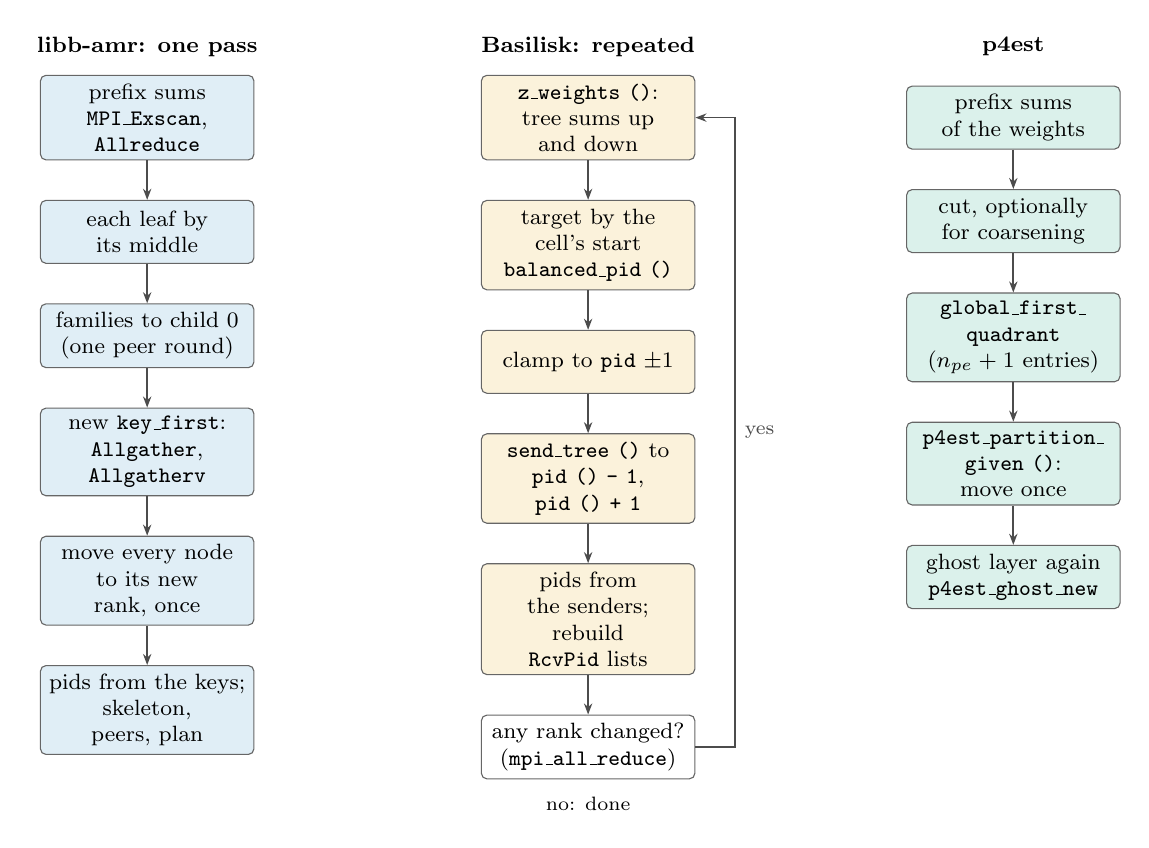
\begin{tikzpicture}[node distance=5mm and 4mm]
    \node[font=\footnotesize\bfseries] at (0,0.9) {libb-amr: one pass};
    \node[box=r0!12] (a1) at (0,0) {prefix sums\\\fn{MPI\_Exscan},
      \fn{Allreduce}};
    \node[box=r0!12, below=of a1] (a2) {each leaf by its middle};
    \node[box=r0!12, below=of a2] (a3) {families to child 0\\(one peer
      round)};
    \node[box=r0!12, below=of a3] (a4) {new \fn{key\_first}:\\
      \fn{Allgather}, \fn{Allgatherv}};
    \node[box=r0!12, below=of a4] (a5) {move every node\\to its new rank,
      once};
    \node[box=r0!12, below=of a5] (a6) {pids from the keys;\\skeleton, peers,
      plan};
    \foreach \u/\v in {a1/a2, a2/a3, a3/a4, a4/a5, a5/a6}
      \draw[flow] (\u) -- (\v);

    \node[font=\footnotesize\bfseries] at (5.6,0.9) {Basilisk:
      repeated};
    \node[box=r1!14] (b1) at (5.6,0) {\fn{z\_weights ()}:\\tree sums up and
      down};
    \node[box=r1!14, below=of b1] (b2) {target by the cell's start\\
      \fn{balanced\_pid ()}};
    \node[box=r1!14, below=of b2] (b3) {clamp to \fn{pid} $\pm 1$};
    \node[box=r1!14, below=of b3] (b4) {\fn{send\_tree ()} to\\\fn{pid () - 1},
      \fn{pid () + 1}};
    \node[box=r1!14, below=of b4] (b5) {pids from the senders;\\rebuild
      \fn{RcvPid} lists};
    \node[box=white, below=of b5] (b6) {any rank changed?\\(\fn{mpi\_all\_reduce})};
    \foreach \u/\v in {b1/b2, b2/b3, b3/b4, b4/b5, b5/b6}
      \draw[flow] (\u) -- (\v);
    \draw[flow] (b6.east) -- ++(0.5,0) |- node[pos=0.25, right,
      font=\scriptsize] {yes} (b1.east);
    \node[font=\scriptsize, below=1mm of b6] {no: done};

    \node[font=\footnotesize\bfseries] at (11.0,0.9) {p4est};
    \node[box=r2!14] (c1) at (11.0,0) {prefix sums\\of the weights};
    \node[box=r2!14, below=of c1] (c2) {cut, optionally\\for coarsening};
    \node[box=r2!14, below=of c2] (c3) {\fn{global\_first\_}\\\fn{quadrant}\\($n_{pe}+1$ entries)};
    \node[box=r2!14, below=of c3] (c4) {\fn{p4est\_partition\_}\\\fn{given ()}: move once};
    \node[box=r2!14, below=of c4] (c5) {ghost layer again\\
      \fn{p4est\_ghost\_new}};
    \foreach \u/\v in {c1/c2, c2/c3, c3/c4, c4/c5}
      \draw[flow] (\u) -- (\v);
  \end{tikzpicture}
  \caption{The three pipelines side by side. libb-amr and p4est cut and
    move once with a table of first keys; Basilisk loops on moves of one
    rank until nothing changes.}
  \label{fig:pipelines}
\end{figure}

% algorithms.tex: the pseudo-code of partition-methods.tex (\input there)
% ======================================================================
\clearpage
\section{Algorithms}
\label{sec:algorithms}

The methods as pseudo-code, in the notation of section~\ref{sec:defs}:
$n_{pe}$ processes, $me$ this one; $\mathcal{L}_{me}$ my own leaves in curve
order, $w_q$ their weights; $\mathrm{key}(p) = M(p)$ the Morton key;
$\mathrm{pid}(p) = \rho(p)$ the owner a node records; $N(p)$ the
neighbourhood of definition~\ref{def:nbhd}. \textsc{Exchange} (algorithm~\ref{alg:exch})
is the only point-to-point primitive libb-amr uses.

The libb-amr algorithms follow \fn{tree-mpi.c} as it is. The Basilisk ones
follow \fn{balance.h} and \fn{tree-mpi.h} as read for this note (through a
web extraction), simplified where marked. The p4est one is from its paper
\cite{p4est} and from memory of its source, not checked here. NBX is from
\cite{nbx}.

% ----------------------------------------------------------------------
\subsection{libb-amr}

\begin{algorithm}[H]
  \caption{\fn{tree\_mpi\_repartition ($w$)}: the cut, then one move}
  \label{alg:repart}
  \begin{algorithmic}[1]
    \Require my own leaves $\mathcal{L}_{me}$ (contiguous on the curve), $w_q
      > 0$ or $w \equiv 1$; the partition table $K^{old}$
      (\fn{key\_first})
    \Ensure every node on its new owner; skeleton, peers and plan rebuilt
    \State $(n, W, b) \gets \textsc{Allreduce}_{+}(|\mathcal{L}_{me}|,
      \sum_q w_q, |\{q : w_q \le 0\}|)$ \Comment{doubles}
    \If{$b > 0$}
      \State \Return $-1$ \Comment{on every rank: nothing changed}
    \EndIf
    \State $(n_{<}, W_{<}) \gets \textsc{Exscan}_{+}(|\mathcal{L}_{me}|,
      \sum_q w_q)$ \Comment{0 on rank 0}
    \For{$q \in \mathcal{L}_{me}$, in curve order}
      \State $r_q \gets \textsc{LeafRank}(W_{<}, w_q, W, n_{pe})$;\quad
        $W_{<} \gets W_{<} + w_q$
    \EndFor
    \State \textsc{KeepFamilies}$(r)$ \Comment{algorithm~\ref{alg:family}}
    \State $K \gets$ \textsc{NewTable}$(r, w)$
      \Comment{the new \fn{key\_first}, loads, imbalance}
    \State \textsc{Migrate}$(K^{old}, K)$ \Comment{algorithm~\ref{alg:migrate}}
    \For{every node $p$ held here}
      \State $\mathrm{pid}(p) \gets \textsc{Owner}(p, K)$
        \Comment{algorithm~\ref{alg:owner}}
    \EndFor
    \State \textsc{SkeletonAndPlan}() \Comment{algorithm~\ref{alg:skeleton};
      every scalar marked stale}
    \State \Return the number of nodes sent
    \Statex
    \Function{LeafRank}{$W_{<}, w, W, n_{pe}$}
      \State \Return $\min\big(n_{pe} - 1, \lfloor n_{pe}\,(W_{<} + w/2) / W \rfloor\big)$
        \Comment{in integers for unit weights}
    \EndFunction
    \Statex
    \Function{NewTable}{$r, w$} \Comment{section~\ref{sec:table}}
      \State $z \gets \textsc{Allgather}(r_{last})$ \Comment{$r$ of my
        last leaf, $-1$ if none}
      \State $\ell \gets -1$
      \For{$o = 0 \ldots n_{pe}-1$}
        \State $c_o \gets \max(0, z_o - \ell)$;\quad \textbf{if} $o =
          me$ \textbf{then} $\ell_{me} \gets \ell$;\quad $\ell \gets
          \max(\ell, z_o)$
      \EndFor
      \For{$s = \ell_{me} + 1 \ldots r_{last}$}
        \State $q \gets$ my first leaf with $r_q \ge s$;\quad $e_s \gets
          (\mathrm{key}(q), W(q), n(q))$ \Comment{$W(q)$, $n(q)$: before $q$}
      \EndFor
      \State $e \gets \textsc{Allgatherv}(e, c)$ \Comment{in the order of
        $s$; $\sum_o c_o \le n_{pe}$}
      \State $(K_s, W_s, n_s) \gets e_s$ for $s < \sum_o c_o$, $(\infty, W, n)$
        after;\quad $K_0 \gets 0$
      \State $\lambda_s \gets W_{s+1} - W_s$;\quad \fn{leaf\_first}$_s
        \gets n_s$
      \State \Return $K$
    \EndFunction
  \end{algorithmic}
\end{algorithm}

\begin{algorithm}[H]
  \caption{\textsc{KeepFamilies}$(r)$: a family of leaves goes whole to
    its child~0's rank}
  \label{alg:family}
  \begin{algorithmic}[1]
    \State $T \gets \emptyset$ \Comment{what I tell my peers}
    \For{$q \in \mathcal{L}_{me}$ that is child 0 of a parent $u$ whose
      $2^D$ children are all leaves}
      \For{the siblings of $q$ that follow it in $\mathcal{L}_{me}$}
        \State $r_{sib} \gets r_q$ \Comment{mine: no message}
      \EndFor
      \If{a sibling of $q$ has $\mathrm{pid} \ne me$}
        \Comment{the family is split}
        \State $T \gets T \cup \{(u, r_q)\}$
      \EndIf
    \EndFor
    \State $R \gets \textsc{Exchange}(\text{peers}, T \text{ to each},
      \text{peers})$ \Comment{one round, peers only}
    \For{$(u, s) \in R$}
      \For{$q \in \mathcal{L}_{me}$ with $\mathrm{parent}(q) = u$}
        \State $r_q \gets s$
      \EndFor
    \EndFor
  \end{algorithmic}
\end{algorithm}

\begin{algorithm}[H]
  \caption{\textsc{Migrate}$(K^{old}, K)$: every node to its new owner,
    in one round}
  \label{alg:migrate}
  \begin{algorithmic}[1]
    \State $to \gets \{\textsc{Owner}(p, K) : \mathrm{pid}(p) = me\} \setminus
      \{me\}$ \Comment{sorted, unique}
    \State $from \gets \{o : \textsc{Owner}(K_{me}, K^{old}) \le o \le
      \textsc{Owner}(K_{me+1} - 1, K^{old}),\; o \ne me,\; K^{old}_o <
      K^{old}_{o+1}\}$
    \Statex \Comment{the old owners of my new piece: a contiguous range of
      ranks}
    \For{every node $p$ with $\mathrm{pid}(p) = me$, $s \gets
      \textsc{Owner}(p, K) \ne me$}
      \State append to $box_s$: index of $p$, leaf or not, the block of
        every scalar in use
      \For{$x \in N(p)$}
        \State append to $box_s$: index of $x$, leaf or not
          \Comment{structure only}
      \EndFor
    \EndFor
    \State $in \gets \textsc{Exchange}(to, box, from)$
    \For{each record $(x, \text{leaf}, \text{data?})$ in $in$}
      \State \fn{tree\_insert}$(x, \text{leaf})$ \Comment{with its missing
        ancestors and their families}
      \If{data}
        \State \fn{activate\_one}$(x)$; copy the blocks in
      \EndIf
    \EndFor
  \end{algorithmic}
\end{algorithm}

\begin{algorithm}[H]
  \caption{\textsc{Owner}$(p, K)$ (\fn{tree\_partition\_owner}): the
    rank whose piece holds $p$, no message}
  \label{alg:owner}
  \begin{algorithmic}[1]
    \State $k \gets \mathrm{key}(p)$;\quad $lo \gets 0$;\quad $hi \gets n_{pe}$
      \Comment{invariant $K_{lo} \le k < K_{hi}$}
    \While{$hi - lo > 1$}
      \State $mid \gets \lfloor (lo + hi)/2 \rfloor$
      \If{$K_{mid} \le k$} $lo \gets mid$ \Else\ $hi \gets mid$ \EndIf
    \EndWhile
    \State \Return $lo$ \Comment{an empty rank has $K_s = K_{s+1}$: passed
      over}
  \end{algorithmic}
\end{algorithm}

\begin{algorithm}[H]
  \caption{\textsc{Exchange}$(to, out, from)$ (\fn{exchange\_with}): point
    to point, both sides name each other}
  \label{alg:exch}
  \begin{algorithmic}[1]
    \For{$f \in from$} \State \textsc{Irecv}(size $n_f$ from $f$) \EndFor
    \For{$t \in to$} \State \textsc{Isend}(size $|out_t|$ to $t$)
      \Comment{0 too: the receiver waits for it} \EndFor
    \State \textsc{Waitall}
    \For{$f \in from$ with $n_f > 0$} \State \textsc{Irecv}($in_f$, $n_f$
      bytes, from $f$) \EndFor
    \For{$t \in to$ with $|out_t| > 0$} \State \textsc{Isend}($out_t$ to
      $t$) \EndFor
    \State \textsc{Waitall};\quad \Return $in$
  \end{algorithmic}
\end{algorithm}

\begin{algorithm}[H]
  \caption{\textsc{SkeletonAndPlan}() (\fn{skeleton\_and\_plan}): what a
    rank keeps and exchanges}
  \label{alg:skeleton}
  \begin{algorithmic}[1]
    \State $O \gets \{p : \mathrm{pid}(p) = me\}$
    \State mark $O$, the ancestors of $O$, and $N(p)$ for every $p \in O$
      \Comment{1. the skeleton}
    \State \fn{tree\_forget} every unmarked leaf;\; prune every unmarked
      subtree
    \State $peers \gets \{\mathrm{pid}(x) : x \in N(p), p \in O\} \setminus
      \{me\}$ \Comment{2. symmetric, by 2:1 balance}
    \State $(depth, depth_{min}) \gets \textsc{Allreduce}_{\max}$ of my own
      leaves' levels
    \State $recv \gets$ for each kind (restrict, ghosts, faces) and level:
      the nodes of $N(O)$ owned by a peer \Comment{3. the plan}
    \State $asked \gets \textsc{Exchange}(peers, recv, peers)$;\quad
      $send \gets asked$ \Comment{I send what my peers ask}
    \State give blocks to every family with an active member
      \Comment{4. the blocks}
  \end{algorithmic}
\end{algorithm}

\textbf{Collectives in one repartition:} 1 \textsc{Allreduce} of the
totals with the weight check, 1 \textsc{Exscan}, 1 \textsc{Allgather} and
1 \textsc{Allgatherv} (\textsc{NewTable}), 1 \textsc{Allreduce} of the
levels; then 3 point-to-point rounds (families, migration, plan).

\begin{algorithm}[H]
  \caption{The end of \fn{adapt\_wavelet ()} on a distributed tree: when
    to repartition (section~\ref{sec:when})}
  \label{alg:when}
  \begin{algorithmic}[1]
    \State \textsc{SkeletonAndPlan}() \Comment{after refining and coarsening}
    \State $split \gets [\exists$ a family of leaves with a leaf of mine and
      one of another rank$]$
    \State $(a, b, N, n_{\max}, split) \gets \textsc{Allreduce}(a, b,
      |\mathcal{L}_{me}|, |\mathcal{L}_{me}|, split)$ \Comment{3 sums, 2
      maxima}
    \If{$split$ \textbf{or} $n_{\max} > \max(\eta_{\max} N / n_{pe},\;
      \lceil N / n_{pe} \rceil + 2^D - 1)$}
      \State \fn{tree\_mpi\_repartition}(1) \Comment{algorithm~\ref{alg:repart}}
    \EndIf
    \State \Return $(a, b)$ \Comment{divided, merged: the whole tree's}
  \end{algorithmic}
\end{algorithm}

\begin{algorithm}[H]
  \caption{Rabenseifner's allreduce \cite{rabenseifner, thakur}, $p =
    2^k$ ranks, a vector $x$ of $n$ bytes}
  \label{alg:rabenseifner}
  \begin{algorithmic}[1]
    \State $[a, b) \gets [0, n)$ \Comment{the window this rank works on}
    \For{$d = p/2, p/4, \ldots, 1$} \Comment{reduce-scatter, recursive halving}
      \State $m \gets (a + b)/2$;\quad $t \gets r \oplus d$
      \If{$r \mathbin{\&} d = 0$}
        \State send $x[m, b)$ to $t$, receive $y$ for $[a, m)$;\quad $b
          \gets m$
      \Else
        \State send $x[a, m)$ to $t$, receive $y$ for $[m, b)$;\quad $a
          \gets m$
      \EndIf
      \State $x[a, b) \gets x[a, b) \oplus y$ \Comment{$n d / p$ bytes
        combined}
    \EndFor
    \Statex \Comment{$x[a, b)$ is block $r$, reduced over all $p$ ranks}
    \For{$d = 1, 2, \ldots, p/2$} \Comment{allgather, recursive doubling}
      \State $t \gets r \oplus d$;\quad send $x[a, b)$ to $t$, receive the
        partner's window next to it
      \State $[a, b) \gets$ the union, twice as long
    \EndFor
    \State \Return $x$ \Comment{$2\log_2 p\,\alpha + 2\frac{p-1}{p}n\beta +
      \frac{p-1}{p}n\gamma$}
  \end{algorithmic}
\end{algorithm}

% ----------------------------------------------------------------------
\subsection{Basilisk}

Simplified: the pseudo-code keeps the order of the steps and the
messages, not every flag. \fn{NEWPID} is a per-cell field holding the
target (1-based, 0 for none).

\begin{algorithm}[H]
  \caption{\fn{mpi\_boundary\_update ()}: balance by repeated passes}
  \label{alg:bas-update}
  \begin{algorithmic}[1]
    \State \fn{mpi\_boundary\_update\_buffers ()}
      \Comment{the \fn{RcvPid} lists, algorithm~\ref{alg:bas-buffers}}
    \While{\textsc{Balance}$(w)$} \Comment{each pass moves cells by one rank
      at most}
    \EndWhile
  \end{algorithmic}
\end{algorithm}

\begin{algorithm}[H]
  \caption{\textsc{Balance}$(w)$ (\fn{balance ()}): one pass, cells to
    $\mathrm{pid} \pm 1$}
  \label{alg:bas-balance}
  \begin{algorithmic}[1]
    \State $(n_{max}, n_{min}) \gets \textsc{Allreduce}_{\max,\min}$(my
      leaf count)
    \If{the counts are balanced enough}
      \State \Return false
    \EndIf
    \State $(cw, tl) \gets \textsc{ZWeights}(w)$
      \Comment{algorithm~\ref{alg:zweights}; $tl$ by one
      \textsc{Allreduce}}
    \For{each local cell $c$}
      \State $t \gets \min\big(\lfloor cw_c / (tl / n_{pe}) \rfloor, n_{pe} - 1\big)$
        \Comment{\fn{balanced\_pid}: from the cell's start}
      \State $t \gets \mathrm{clamp}(t, \mathrm{pid}(c) - 1, \mathrm{pid}(c)
        + 1)$
      \If{$t \ne \mathrm{pid}(c)$} \State $\fn{NEWPID}(c) \gets t + 1$ \EndIf
    \EndFor
    \State halo exchange of \fn{NEWPID}, level by level
      \Comment{\fn{boundary\_iterate (level, ...)}}
    \State \fn{send\_tree} (cells for $me - 1$) to $me - 1$;\;
      \fn{send\_tree} (cells for $me + 1$) to $me + 1$
    \State \fn{receive\_tree} from $me - 1$ and from $me + 1$
      \Comment{the cells, their data and new pids}
    \For{each cell $c$ with a \fn{NEWPID}} \State $\mathrm{pid}(c) \gets
      \fn{NEWPID}(c) - 1$ \EndFor
    \State coarse cells without one: the pid of their parent
    \State flag border cells again
    \State $changed \gets \textsc{Allreduce}_{\max}$(a pid changed here)
    \If{$changed$} \State \fn{mpi\_boundary\_update\_buffers ()} \EndIf
    \State \Return $changed$
  \end{algorithmic}
\end{algorithm}

\begin{algorithm}[H]
  \caption{\textsc{ZWeights}$(w)$ (\fn{z\_weights}): the weight before each
    cell, through the tree}
  \label{alg:zweights}
  \begin{algorithmic}[1]
    \For{level $l = depth \ldots 0$} \Comment{up: subtree weights}
      \For{each local cell $c$ at level $l$}
        \State $sw_c \gets (c \text{ a leaf} \; ? \; w_c : \sum_{\text{children
          } h} sw_h)$
      \EndFor
      \State halo exchange of $sw$ at level $l$
        \Comment{\fn{boundary\_iterate (restriction, ...)}}
    \EndFor
    \State $tl \gets \textsc{Allreduce}_{\max}(me = 0 \; ? \; sw_{root} :
      -1)$ \Comment{the only collective}
    \State $cw_{root} \gets 0$
    \For{level $l = 0 \ldots depth - 1$} \Comment{down: offsets}
      \For{each local cell $c$ at level $l$ with children $h_0 \ldots
        h_{2^D-1}$}
        \State $cw_{h_i} \gets cw_c + \sum_{j<i} sw_{h_j}$
      \EndFor
      \State halo exchange of $cw$ at level $l+1$
    \EndFor
    \State \Return $(cw, tl)$
  \end{algorithmic}
\end{algorithm}

\begin{algorithm}[H]
  \caption{\fn{mpi\_boundary\_update\_buffers ()}: the send and receive
    lists, from the pids}
  \label{alg:bas-buffers}
  \begin{algorithmic}[1]
    \State free the \fn{RcvPid} lists (\fn{mpi\_level},
      \fn{mpi\_level\_root}, \fn{restriction})
    \For{each cell $c$ (\fn{foreach\_cell})}
      \If{$c$ is local and has a neighbour with pid $s \ne me$}
        \State add $c$ to the send list for $s$ at $c$'s level
      \EndIf
      \If{$c$ is remote (pid $s \ne me$) and next to a local cell}
        \State add $c$ to the receive list from $s$
          \Comment{\fn{rcv\_pid\_pointer}: one \fn{Rcv} per pid seen}
      \EndIf
    \EndFor
    \State coarsen away the remote cells no list uses
      \Comment{``we remove unused cells''}
  \end{algorithmic}
\end{algorithm}

% ----------------------------------------------------------------------
\subsection{p4est}

From the paper \cite{p4est} and memory of the source, not checked here.
p4est keeps \fn{global\_first\_quadrant} ($G$, $n_{pe}+1$ counts, the global
index of each rank's first quadrant) on every rank.

\begin{algorithm}[H]
  \caption{\fn{p4est\_partition ($w$, for\_coarsening)}}
  \label{alg:p4est}
  \begin{algorithmic}[1]
    \State $\omega \gets \textsc{Allgather}(\sum_{q \in \mathcal{L}_{me}} w_q)$
      \Comment{$n_{pe}$ local sums, on every rank}
    \State $\Omega_s \gets \sum_{t < s} \omega_t$ \Comment{prefix, computed
      locally}
    \State for each rank $s$: its new first quadrant is the first $q$ with
      prefix weight $\ge s\,\Omega_{n_{pe}} / n_{pe}$
    \Statex \Comment{each rank finds the cuts that fall in its own piece and
      shares them}
    \If{for\_coarsening}
      \State move each cut off a family of siblings
        \Comment{\fn{p4est\_partition\_for\_coarsening}: a family whole on
        one rank}
    \EndIf
    \State $G' \gets$ the new first quadrants \Comment{$n_{pe}+1$ entries}
    \State \textsc{PartitionGiven}$(G, G')$
    \State \fn{p4est\_ghost\_new ()} \Comment{the ghost layer again}
    \Statex
    \Function{PartitionGiven}{$G, G'$}
      \Comment{\fn{p4est\_partition\_given}}
      \For{each rank $s$ with $[G'_s, G'_{s+1}) \cap [G_{me}, G_{me+1}) \ne
        \emptyset$, $s \ne me$}
        \State \textsc{Isend} the quadrants of that intersection to $s$
      \EndFor
      \For{each rank $o$ with $[G_o, G_{o+1}) \cap [G'_{me}, G'_{me+1}) \ne
        \emptyset$, $o \ne me$}
        \State \textsc{Irecv} that intersection from $o$
          \Comment{sizes known from $G, G'$: no size round}
      \EndFor
      \State \textsc{Waitall};\; assemble the new local range in order;\;
        $G \gets G'$
    \EndFunction
  \end{algorithmic}
\end{algorithm}

Compared with algorithm~\ref{alg:repart}: the same cut and the same single
move. p4est counts quadrants, so $G, G'$ give every message's size and
the size round of \textsc{Exchange} is not needed; libb-amr also sends
$N(p)$ with each node, whose size only the sender knows.

% ----------------------------------------------------------------------
\subsection{NBX: a sparse exchange without knowing the senders}

Hoefler, Siebert and Lumsdaine \cite{nbx}. It replaces \textsc{Exchange}
when a rank knows whom it sends to but not who sends to it, so no table
and no \textsc{Alltoall} of sizes is needed.

\begin{algorithm}[H]
  \caption{\textsc{NBX}$(to, out)$: receive from whoever sends}
  \label{alg:nbx}
  \begin{algorithmic}[1]
    \For{$t \in to$}
      \State \textsc{Issend}$(out_t \to t)$ \Comment{synchronous: completes
        only once matched by a receive}
    \EndFor
    \State $in \gets \emptyset$;\quad $barrier \gets$ none
    \Loop
      \If{\textsc{Iprobe}(ANY\_SOURCE) finds a message from $s$}
        \State $in_s \gets \textsc{Recv}$(its size, from $s$)
      \EndIf
      \If{$barrier = $ none}
        \If{\textsc{Testall}(my \textsc{Issend}s)}
          \Comment{all my messages are received}
          \State $barrier \gets \textsc{Ibarrier}()$
        \EndIf
      \ElsIf{\textsc{Test}$(barrier)$}
        \State \Return $in$ \Comment{every rank's sends are matched:
          nothing in flight}
      \EndIf
    \EndLoop
  \end{algorithmic}
\end{algorithm}

\textbf{Why it is correct.} A rank enters the barrier only when every
message it sent has been received. So when the barrier completes, every
message of every rank has been received, and none can still arrive. The
cost is the messages themselves plus one non-blocking barrier,
$O(\log n_{pe})$.

\textbf{In libb-amr} it would replace the $from$ set of \textsc{Migrate}
(algorithm~\ref{alg:migrate}, found from $K^{old}$) and so allow dropping
the table, with the pids then told by the senders as in Basilisk.


% ======================================================================
\section{Side by side}

\begin{center}
\small
\begin{tabular}{>{\raggedright}p{3.2cm} >{\raggedright}p{5.6cm}
  >{\raggedright\arraybackslash}p{5.6cm}}
  \toprule
  & \textbf{Basilisk} & \textbf{libb-amr} \\
  \midrule
  owner of a nearby cell & \fn{cell.pid}, on local and halo cells &
    \fn{node->pid}, on skeleton nodes: the same idea \\
  owner of any index & not needed & \fn{key\_first} ($n_{pe}+1$ keys),
    binary search \\
  the cut & prefix weights by tree sums, neighbour exchanges only &
    \fn{MPI\_Exscan} and \fn{MPI\_Allreduce} \\
  moving cells & to rank $\pm 1$, repeated until no change & one pass,
    straight to the final rank \\
  new partition table & none & \fn{MPI\_Allgather} of an int,
    \fn{MPI\_Allgatherv} of $n_{pe}$ entries \\
  when to balance & every \fn{mpi\_boundary\_update ()}, until no change &
    when a family is split or a rank is above $\eta_{\max}$ and a cut's
    bound \\
  pids after a move & told by the sending neighbour & from the new keys \\
  families of siblings & no rule found in the files read & never split
    (child 0's rank) \\
  weights & \fn{balance\_weights}; \fn{LB\_AUTO} measures busy time &
    given by the caller \\
  halo lists & \fn{RcvPid}, per neighbour and level & \fn{TreeMpiPlan},
    per peer, kind and level \\
  what a rank holds & local, halo, ancestors; unused halo coarsened away &
    the skeleton; inactive nodes without blocks \\
  \bottomrule
\end{tabular}
\end{center}

\textbf{Messages in one libb-amr repartition:} 1 \fn{MPI\_Exscan}, 2
\fn{MPI\_Allreduce} (the totals with the weight check, the levels), 1
\fn{MPI\_Allgather}, 1 \fn{MPI\_Allgatherv}, one peer round for split
families, one migration round, then the rounds of \fn{distribute\_again
()} for the skeleton and plan.

\textbf{Where Basilisk's details come from.} \fn{src/grid/balance.h} and
\fn{src/grid/tree-mpi.h}, read through a web extraction rather than a
byte-exact copy: check the quoted lines against the source before relying
on them.

% ======================================================================
\begin{thebibliography}{99}
\small
\bibitem{warren} M.~S.~Warren, J.~K.~Salmon. A parallel hashed oct-tree
  N-body algorithm. \emph{Supercomputing '93}, 1993.
\bibitem{pilkington} J.~R.~Pilkington, S.~B.~Baden. Dynamic partitioning
  of non-uniform structured workloads with spacefilling curves.
  \emph{IEEE Trans.\ Parallel Distrib.\ Syst.} 7~(3), 1996.
\bibitem{aluru} S.~Aluru, F.~E.~Sevilgen. Parallel domain decomposition
  and load balancing using space-filling curves. \emph{HiPC}, 1997.
\bibitem{pinar} A.~Pinar, C.~Aykanat. Fast optimal load balancing
  algorithms for 1D partitioning. \emph{J.\ Parallel Distrib.\ Comput.}
  64~(8), 2004.
\bibitem{p4est} C.~Burstedde, L.~C.~Wilcox, O.~Ghattas. p4est: scalable
  algorithms for parallel adaptive mesh refinement on forests of
  octrees. \emph{SIAM J.\ Sci.\ Comput.} 33~(3), 2011.
\bibitem{rabenseifner} R.~Rabenseifner. Optimization of collective
  reduction operations. \emph{ICCS}, LNCS 3036, 2004.
\bibitem{rabtraff} R.~Rabenseifner, J.~L.~Tr\"aff. More efficient
  reduction algorithms for non-power-of-two number of processors in
  message-passing parallel systems. \emph{EuroPVM/MPI}, LNCS 3241, 2004.
\bibitem{thakur} R.~Thakur, R.~Rabenseifner, W.~Gropp. Optimization of
  collective communication operations in MPICH. \emph{Int.\ J.\ High
  Perform.\ Comput.\ Appl.} 19~(1), 2005.
\bibitem{chan} E.~Chan, M.~Heimlich, A.~Purkayastha, R.~van~de~Geijn.
  Collective communication: theory, practice, and experience.
  \emph{Concurr.\ Comput.: Pract.\ Exper.} 19~(13), 2007.
\bibitem{patarasuk} P.~Patarasuk, X.~Yuan. Bandwidth optimal all-reduce
  algorithms for clusters of workstations. \emph{J.\ Parallel Distrib.\
  Comput.} 69~(2), 2009.
\bibitem{bruck} J.~Bruck, C.-T.~Ho, S.~Kipnis, E.~Upfal, D.~Weathersby.
  Efficient algorithms for all-to-all communications in multiport
  message-passing systems. \emph{IEEE Trans.\ Parallel Distrib.\ Syst.}
  8~(11), 1997.
\bibitem{nbx} T.~Hoefler, C.~Siebert, A.~Lumsdaine. Scalable
  communication protocols for dynamic sparse data exchange. \emph{PPoPP},
  2010.
\bibitem{basilisk} S.~Popinet. Basilisk, \url{http://basilisk.fr},
  \fn{src/grid/balance.h}, \fn{src/grid/tree-mpi.h}.
\end{thebibliography}

\noindent\footnotesize The references are cited from memory, not checked
against the publications: verify them before citing this note.

\end{document}
